% !TeX program = lualatex
% Relatório de atividades desenvolvidas — ICTSR/UFSCar.
\documentclass[12pt,a4paper]{article}

\usepackage{fontspec}
\usepackage{polyglossia}
\setdefaultlanguage[variant=brazilian]{portuguese}
\setmainfont{Fira Sans}
\setsansfont{Fira Sans}
\setmonofont{Fira Mono}[Scale=MatchLowercase]

\usepackage[a4paper,margin=2.5cm,headheight=15pt]{geometry}
\usepackage{setspace}
\onehalfspacing
\usepackage{microtype}
\usepackage{graphicx}
\graphicspath{{figures/}}
\usepackage{booktabs,longtable,tabularx,array,multirow}
\usepackage[table]{xcolor}
\usepackage{siunitx}
\sisetup{
  mode=match,
  output-decimal-marker={,},
  group-separator={.},
  group-minimum-digits=4
}
\usepackage{amsmath}
\usepackage{unicode-math}
\setmathfont{Fira Math}
\usepackage{enumitem}
\usepackage{caption}
\usepackage{float}
\usepackage[section]{placeins}
\usepackage{needspace}
\usepackage{pdflscape}
\usepackage{listings}
\usepackage{tikz}
\usetikzlibrary{arrows.meta,backgrounds,calc,fit,matrix,positioning,shapes.geometric}
\usepackage{pgfplots}
\pgfplotsset{compat=1.18}
\usepgfplotslibrary{groupplots}
\usepackage{fancyhdr}
\usepackage{titlesec}
\usepackage[hidelinks,unicode]{hyperref}
\usepackage[num]{abntex2cite}
% A opção explícita evita definições legadas incompatíveis com Unicode do
% cleveref para o português; os nomes usados no texto são definidos abaixo.
\usepackage[english,noabbrev,nameinlink]{cleveref}

\definecolor{azul}{HTML}{174A7E}
\definecolor{azulclaro}{HTML}{E7F0F8}
\definecolor{verde}{HTML}{2F7D4A}
\definecolor{verdeclaro}{HTML}{E8F4EB}
\definecolor{laranja}{HTML}{B35A16}
\definecolor{laranjaclaro}{HTML}{FFF0E3}
\definecolor{vermelho}{HTML}{A22A2A}
\definecolor{vermelhoclaro}{HTML}{FBE8E8}
\definecolor{cinza}{HTML}{606770}
\definecolor{cinzaclaro}{HTML}{F1F3F5}

\titleformat{\section}{\Large\bfseries\color{azul}}{\thesection}{0.7em}{}
\titleformat{\subsection}{\large\bfseries\color{azul}}{\thesubsection}{0.7em}{}
\titleformat{\subsubsection}{\normalsize\bfseries}{\thesubsubsection}{0.7em}{}
% Evita títulos órfãos: uma seção reserva espaço para comportar também uma
% subseção imediatamente seguinte e o começo de seu texto; os níveis inferiores
% reservam algumas linhas do conteúdo correspondente. A barreira de placeins
% acima impede, adicionalmente, que uma figura da seção anterior ultrapasse o
% novo título.
\AddToHook{cmd/section/before}{\Needspace{12\baselineskip}}
\AddToHook{cmd/subsection/before}{\Needspace{5\baselineskip}}
\AddToHook{cmd/subsubsection/before}{\Needspace{4\baselineskip}}
\clubpenalty=10000
\widowpenalty=10000
\displaywidowpenalty=10000
\setlength{\parindent}{1.1cm}
\setlength{\parskip}{0.15em}
\setlist{itemsep=0.2em,topsep=0.4em}
\renewcommand{\arraystretch}{1.18}

\pagestyle{fancy}
\fancyhf{}
\fancyhead[L]{\small Relatório final de atividades desenvolvidas — ICTSR}
\fancyhead[R]{\small Gabriel Kusumota Nadalin}
\fancyfoot[C]{\thepage}
\renewcommand{\headrulewidth}{0.3pt}

\hypersetup{
  pdftitle={Montagem de bancada de testes com servidor de acesso remoto para engenharia reversa do softmodem slmodem},
  pdfauthor={Gabriel Kusumota Nadalin},
  pdfsubject={Relatório final de atividades desenvolvidas — ICTSR/UFSCar},
  pdfkeywords={ICTSR, slmodem, V.90, E1, SIP, RTP, engenharia reversa}
}

\newcolumntype{Y}{>{\raggedright\arraybackslash}X}
\newcolumntype{C}[1]{>{\centering\arraybackslash}p{#1}}
\newcommand{\slmodem}{\textit{slmodem}}
\newcommand{\dsplibs}{\texttt{dsplibs.o}}
\newcommand{\ok}{\cellcolor{verdeclaro}\textcolor{verde}{\textbf{Aprovado}}}
\newcommand{\falha}{\cellcolor{vermelhoclaro}\textcolor{vermelho}{\textbf{Não conecta}}}
\newcommand{\na}{\cellcolor{cinzaclaro}\textcolor{cinza}{---}}
\newcommand{\arquivo}[1]{{\def\UrlLeft{}\def\UrlRight{}\path{#1}}}
\newcommand{\repositorio}{%
  \href{https://github.com/gabriel-nadalin/dial-up-bench}{%
    {\def\UrlLeft{}\def\UrlRight{}\nolinkurl{https://github.com/gabriel-nadalin/dial-up-bench}}}}

\crefname{figure}{figura}{figuras}
\crefname{table}{tabela}{tabelas}
\crefname{section}{seção}{seções}
\crefname{appendix}{apêndice}{apêndices}

\lstdefinestyle{codigo}{
  basicstyle=\ttfamily\footnotesize,
  backgroundcolor=\color{cinzaclaro},
  frame=single,
  rulecolor=\color{cinza!40},
  breaklines=true,
  columns=fullflexible,
  keepspaces=true,
  showstringspaces=false,
  xleftmargin=0.4em,
  xrightmargin=0.4em
}
\lstset{style=codigo}

\begin{document}
\hypersetup{pageanchor=false}

\begin{titlepage}
  \begin{center}
    {\large\bfseries UNIVERSIDADE FEDERAL DE SÃO CARLOS\par}
    \vspace{0.25cm}
    {\large Departamento de Computação\par}
    \vspace{0.25cm}
    {\large Programa Institucional de Iniciação Científica e Tecnológica\par}
    {\large Iniciação Científica e Tecnológica sem Remuneração — ICTSR\par}

    \vfill

    {\Large\bfseries\color{azul}
      MONTAGEM DE BANCADA DE TESTES COM SERVIDOR DE ACESSO REMOTO PARA
      ENGENHARIA REVERSA DO SOFTMODEM SLMODEM\par}

    \vspace{1.4cm}
    {\large\bfseries Relatório final de atividades desenvolvidas\par}
    \vspace{0.2cm}
    {\normalsize Projeto encerrado por conclusão do curso de graduação\par}

    \vfill

    \begin{tabular}{rl}
      \textbf{Estudante:} & Gabriel Kusumota Nadalin \\
      \textbf{Curso:} & Bacharelado em Ciência da Computação \\
      \textbf{Orientador:} & Prof. Dr. Paulo Matias \\
      \textbf{Modalidade:} & ICTSR — sem remuneração \\
      \textbf{Vigência registrada:} & 1º de abril a 6 de agosto de 2026 \\
    \end{tabular}

    \vfill
    {São Carlos\par}
    {Setembro de 2026\par}
  \end{center}
\end{titlepage}

\hypersetup{pageanchor=true}
\pagenumbering{roman}

\section*{Identificação e natureza deste relatório}
\addcontentsline{toc}{section}{Identificação e natureza deste relatório}

Este documento relata as atividades desenvolvidas no projeto de ICTSR
\emph{Montagem de bancada de testes com servidor de acesso remoto para engenharia
reversa do softmodem slmodem}. No SAGUI, o projeto teve início em 1º de abril de
2026, previsão original de término em 1º de abril de 2027 e cancelamento aceito
em 6 de agosto de 2026. O cancelamento foi motivado exclusivamente pela conclusão
da graduação e consequente perda do vínculo acadêmico do estudante, cuja colação
de grau estava marcada para 7 de agosto. Não decorreu de abandono, inviabilidade
técnica ou descumprimento do plano.

O documento atende ao relatório das atividades desenvolvidas previsto para o
cancelamento de projetos ICTSR. Como o trabalho avançou mais rápido
que o cronograma anual originalmente proposto, todas as frentes experimentais
previstas foram executadas, inclusive a conexão E1 direta indicada no projeto como
atividade opcional. Ensaios de controle que surgiram durante a investigação são
apresentados junto dos resultados a que dão suporte, sem alterar o objetivo do
projeto.

\begin{table}[H]
\centering
\caption{Identificação administrativa e científica do projeto.}
\label{tab:identificacao}
\begin{tabularx}{\textwidth}{>{\bfseries}p{0.29\textwidth}Y}
\toprule
Modalidade & Iniciação Científica e Tecnológica sem Remuneração (ICTSR) \\
Área & Ciência da Computação \\
Estudante & Gabriel Kusumota Nadalin \\
Orientador & Paulo Matias \\
Título & Montagem de bancada de testes com servidor de acesso remoto para engenharia reversa do softmodem \slmodem \\
Motivo do encerramento & Término da graduação e perda de vínculo acadêmico \\
Situação das atividades & Atividades experimentais previstas integralmente executadas; resultados e artefatos consolidados no repositório do projeto \\
\bottomrule
\end{tabularx}
\end{table}

\clearpage
\section*{Declaração de Uso de IA}
\addcontentsline{toc}{section}{Declaração de Uso de IA}

\begingroup
\tolerance=1000
\setlength{\emergencystretch}{0.5em}
A elaboração deste trabalho contou com o auxílio de ferramentas de inteligência
artificial generativa como suporte instrumental. Utilizaram-se os modelos
\mbox{deepseek-4-flash}, \mbox{deepseek-4-pro} e \mbox{kimi-k3} em conjunto com
os harnesses \mbox{oh-my-pi} e opencode; e o modelo \mbox{gpt-5.6-sol} em
conjunto com o harness codex, especificamente para: (1) revisão bibliográfica;
(2) prototipação de código; (3) verificação de procedimentos experimentais; (4)
consolidação de resultados e sumarização de texto; e (5) revisão ortográfica,
gramatical e de estilo.
\par
\endgroup

É imperativo ressaltar que todo o conteúdo gerado por essas ferramentas foi
submetido a uma rigorosa validação humana, assegurando a precisão factual e a
aderência à literatura especializada. A concepção intelectual, a análise crítica,
a síntese dos dados e a redação final permanecem de inteira responsabilidade do
autor, que validou integralmente o material produzido.

\clearpage
\section*{Resumo}
\addcontentsline{toc}{section}{Resumo}

O \slmodem{} é um modem implementado majoritariamente em software para Linux,
mas seu núcleo de processamento digital de sinais, distribuído como o objeto
binário x86 de 32 bits \dsplibs, não possui código-fonte disponível. Sua
reconstrução por engenharia reversa demanda testes de integração capazes de
estabelecer chamadas reais, especialmente no protocolo V.90, cujo enlace
descendente de até \SI{56000}{bit/s} requer terminação digital na extremidade
servidora. Este projeto construiu e validou uma bancada formada por um servidor de
acesso Cisco AS5300 com modems digitais MICA, um gateway Cisco 2911, um modem USB
de referência, um ATA Grandstream HT503 e uma interface E1 Sangoma. Também foram
desenvolvidos uma ponte entre o \slmodem{} e fluxos PCM, transportes SIP/RTP e E1,
uma ferramenta de sinalização PRI e um orquestrador Python que automatiza chamadas
e verifica tráfego de dados pela porta serial virtual do modem. A validação com o
modem de referência alcançou V.90; o \slmodem{} estabeleceu conexões funcionais de
V.21 a V.90 no E1 direto e no caminho SIP digital, sempre com intercâmbio real de
comandos com o RAS. O caminho SIP que atravessa a conversão analógica entre o Cisco
2911 e o HT503 alcançou V.34, mas não V.90. A comparação controlada e a análise de
capturas mostraram perda adicional de aproximadamente \SI{10.1}{dB} em
\SI{3.8}{kHz}, \SI{21.0}{dB} próximo de \SI{4}{kHz} e desvio de relógio de
\SI{-114.1}{ppm} nesse trecho. A documentação do VINETIC presente no HT503 limita
a atenuação máxima somente até \SI{3.4}{kHz}, e a inspeção do aparelho mostrou
operação PCMA/\SI{8}{kHz} sem modo linear de banda larga habilitado. O resultado principal
é uma bancada funcional, automatizada, documentada e apta a validar a reconstrução
do \dsplibs{} em protocolos até V.90, além da caracterização objetiva da limitação
do caminho analógico empregado.

\noindent\textbf{Palavras-chave:} iniciação tecnológica; engenharia reversa;
softmodem; V.90; E1/PRI; SIP/RTP; processamento digital de sinais.

\clearpage
\tableofcontents
\clearpage
\listoffigures
\clearpage
\listoftables
\clearpage

\pagenumbering{arabic}

\section{Introdução}

Modems de banda de voz constituem um caso particularmente rico de processamento
digital de sinais em tempo real. Em um único enlace aparecem detecção de portadora,
sincronização temporal, equalização adaptativa e cancelamento de eco, problemas
clássicos de processamento digital de sinais \cite{oppenheim2010}, além de codificação
treliça, correção de erros e controle de protocolo. Embora a internet discada tenha
sido substituída comercialmente pela banda larga, seus artefatos permanecem
relevantes tanto para o ensino quanto para a preservação do software e do
conhecimento técnico incorporado a sistemas legados
\cite{dicosmo2017,moshenska2016}.

O \slmodem, originalmente desenvolvido pela Smart Link, separa a interface física
de áudio do processamento de modem. O programa executa em espaço de usuário,
apresenta uma porta serial virtual para comandos AT e dados e consome/produz
amostras de áudio. Entretanto, as rotinas centrais de modulação, demodulação,
sincronização e equalização permaneceram no binário \dsplibs. A disponibilidade
apenas desse objeto x86 de 32 bits impede manutenção plena, auditoria e
portabilidade. O grupo de pesquisa vem reconstruindo o componente incrementalmente,
comparando funções recuperadas com o comportamento do original.

Testes unitários não bastam para estruturas que dependem de estado global, de
temporização e da interação entre diversas fases de treinamento. É necessário
ligar o programa a um servidor de acesso real e observar não apenas a indicação de
portadora, mas o transporte bidirecional de dados. O protocolo V.90 torna esse
requisito mais exigente: o modem servidor deve estar ligado digitalmente à rede
telefônica, enquanto o cliente ocupa a extremidade analógica
\cite{itutv90}. Dois modems clientes convencionais podem testar protocolos
simétricos anteriores, como V.34 \cite{itutv34}, mas não reproduzem o enlace PCM
descendente do V.90.

O projeto surgiu, portanto, para transformar equipamentos disponíveis no laboratório
em uma infraestrutura repetível de integração. O Cisco AS5300 fornece o RAS e os
modems digitais MICA; o Cisco 2911 interliga E1 e portas analógicas; um Conexant
CX93010 serve de referência; o Grandstream HT503 oferece uma ponte SIP/analógica; e
uma interface Sangoma permite alcançar o E1 diretamente. A \cref{fig:ciclo-pesquisa}
resume o papel da bancada no ciclo maior de engenharia reversa.

\begin{figure}[htbp]
\centering
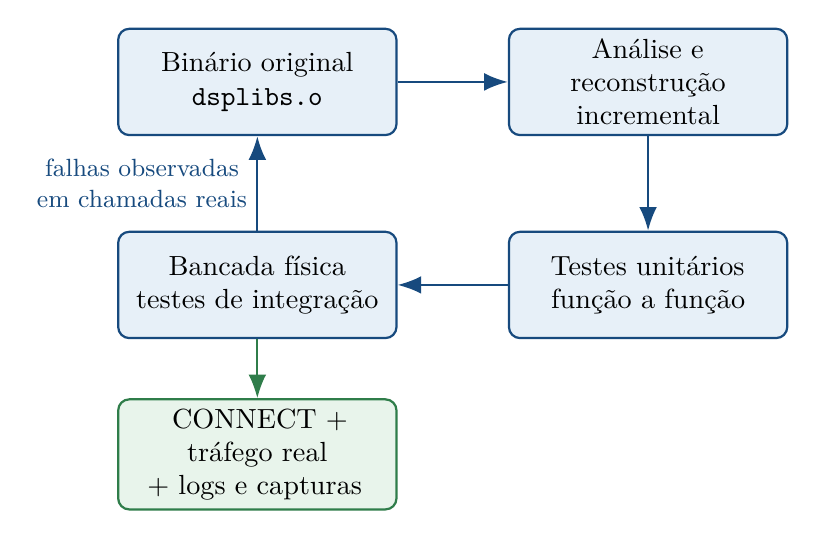
\begin{tikzpicture}[
  node distance=1.2cm and 1.4cm,
  etapa/.style={draw=azul,thick,rounded corners,fill=azulclaro,
                align=center,text width=3.3cm,minimum height=1.35cm},
  seta/.style={-{Latex[length=3mm]},thick,azul}
]
  \node[etapa] (bin) {Binário original\\\dsplibs};
  \node[etapa,right=of bin] (re) {Análise e\\reconstrução incremental};
  \node[etapa,below=of re] (unit) {Testes unitários\\função a função};
  \node[etapa,left=of unit] (bench) {Bancada física\\testes de integração};
  \draw[seta] (bin) -- (re);
  \draw[seta] (re) -- (unit);
  \draw[seta] (unit) -- (bench);
  \draw[seta] (bench) -- node[left,align=center,font=\small]{falhas observadas\\em chamadas reais} (bin);
  \node[draw=verde,fill=verdeclaro,rounded corners,thick,below=0.75cm of bench,
        text width=3.3cm,align=center] (evidence) {CONNECT + tráfego real\\+ logs e capturas};
  \draw[seta,verde] (bench) -- (evidence);
\end{tikzpicture}
\caption{Inserção da bancada no ciclo de reconstrução e validação do núcleo DSP.}
\label{fig:ciclo-pesquisa}
\end{figure}

\section{Objetivos e correspondência com o plano original}

\subsection{Objetivo geral}

O objetivo geral aprovado foi projetar e montar uma bancada de testes de modem
\emph{dial-up} com um Cisco AS5300, capaz de estabelecer conexões V.21, V.22,
V.32bis, V.34 e V.90 com um \emph{softmodem} em computador pessoal, permitindo
coletar logs e executar testes de integração para a engenharia reversa do
\slmodem{}.

\subsection{Objetivos específicos e evidências de execução}

A \cref{tab:objetivos} relaciona cada atividade do projeto original ao produto
observável. Essa matriz é importante porque separa execução de atividade e resultado
experimental: uma tentativa que revela uma limitação do equipamento continua sendo
uma atividade concluída, desde que conduzida, registrada e analisada.

\begin{longtable}{p{0.31\textwidth}p{0.17\textwidth}p{0.44\textwidth}}
\caption{Correspondência entre o plano aprovado e as evidências produzidas.}
\label{tab:objetivos}\\
\toprule
\textbf{Atividade prevista} & \textbf{Situação} & \textbf{Evidência ou produto} \\
\midrule
\endfirsthead
\toprule
\textbf{Atividade prevista} & \textbf{Situação} & \textbf{Evidência ou produto} \\
\midrule
\endhead
Estudar AS5300, Cisco 2911 e opções de sinalização E1 & Concluída & Avaliação de E\&M para a alternativa em FPGA e adoção de CCS/PRI com a placa Sangoma, DAHDI, Wanpipe e libpri. \\
Configurar a interconexão entre AS5300 e 2911 & Concluída & E1 CCS/HDB3/CRC4 e PRI operacional; chamadas encaminhadas aos MICA. \\
Validar a bancada com hardmodem CX93010 & Concluída & Topologia 1 aprovada de V.21 a V.90 com tráfego interativo; PPP/IPCP funcional e sessão V.90 mantida por mais de \SI{24}{h}. \\
Integrar o ATA Grandstream HT503 & Concluída & Chamada SIP, mídia PCMA e discagem FXO funcionais; tráfego de dados aprovado até V.34; limitação de V.90 caracterizada. \\
Adaptar o \slmodem{} para SIP/RTP & Concluída & \arquivo{slmodem_bridge}, \arquivo{rtp_bridge} e orquestração pelo pacote \arquivo{dialbench}. \\
Testar sequencialmente V.21, V.22, V.32bis, V.34 e V.90 & Concluída & Matrizes CSV por topologia; acrescentaram-se V.22bis e V.23 à cobertura. \\
Coletar logs de depuração & Concluída & Logs de modem, RAS e SIP; capturas WAV e resultados quantitativos reprodutíveis. \\
Investigar conexão E1 direta, se viável & Concluída & Topologia 3 implementada com Sangoma, DAHDI e libpri; V.90 aprovado a \SI{56000}{bit/s} descendentes. \\
Documentar procedimentos, topologias e resultados & Concluída & Código, manuais, configurações, matrizes, análise complementar e este relatório. \\
\bottomrule
\end{longtable}

Uma decisão de implementação merece destaque. O projeto inicial considerou a possibilidade
de usar sinalização E\&M para o caso de ser necessário construir uma interface E1
em FPGA, alternativa para a qual era mais simples implementar a sinalização em
hardware e sobre a qual o aluno já havia desenvolvido um protótipo em disciplina
da graduação. No decorrer do trabalho, porém, foi possível adquirir uma placa Sangoma
A102. Com uma interface E1 suportada pela pilha de telefonia do Linux, a opção mais
direta passou a ser CCS com EuroISDN/PRI, disponível nativamente por meio de
DAHDI e libpri. A adoção de PRI, portanto, não decorreu de uma tentativa malsucedida
de encaminhar chamadas com E\&M, mas da escolha da solução mais simples e adequada
ao hardware que se tornou disponível. O objetivo funcional permaneceu o mesmo:
interligar a bancada ao AS5300 e entregar as chamadas aos modems MICA.

\section{Fundamentação técnica}

\subsection{Assimetria do V.90}

O V.90 combina dois mecanismos. No sentido cliente--servidor, emprega modulação
analógica com taxa de até \SI{33600}{bit/s}. No sentido servidor--cliente,
explora o fato de o servidor injetar diretamente palavras PCM na rede digital e
alcança até \SI{56000}{bit/s} \cite{itutv90}. Uma conversão digital--analógica
permanece inevitável na linha do assinante, mas elimina-se uma conversão analógica--digital
no lado servidor. É por isso que a bancada precisa de RAS com acesso E1 e
modems digitais, e não apenas de dois modems clientes.

Durante a fase TRN1d, o servidor transmite uma sequência antipodal de 8 mil
símbolos por segundo. O receptor do \slmodem{} usa, entre outras informações,
a energia próxima da borda da banda para classificar o canal e recuperar
temporização. Isso faz com que um caminho adequado a voz, embora excelente até
\SI{3.4}{kHz}, possa ser inadequado ao V.90.

\subsection{Planos de controle, mídia e dados}

A ligação envolve três planos distintos, mostrados na \cref{fig:planos}. SIP ou
Q.931/PRI estabelece e encerra a chamada; RTP/PCMA ou o canal B E1 transporta
amostras; a porta serial virtual carrega comandos AT antes do \texttt{CONNECT} e
dados depois dele. A separação foi essencial para não interpretar uma chamada SIP
atendida como prova de que o modem treinou corretamente.

\begin{figure}[htbp]
\centering
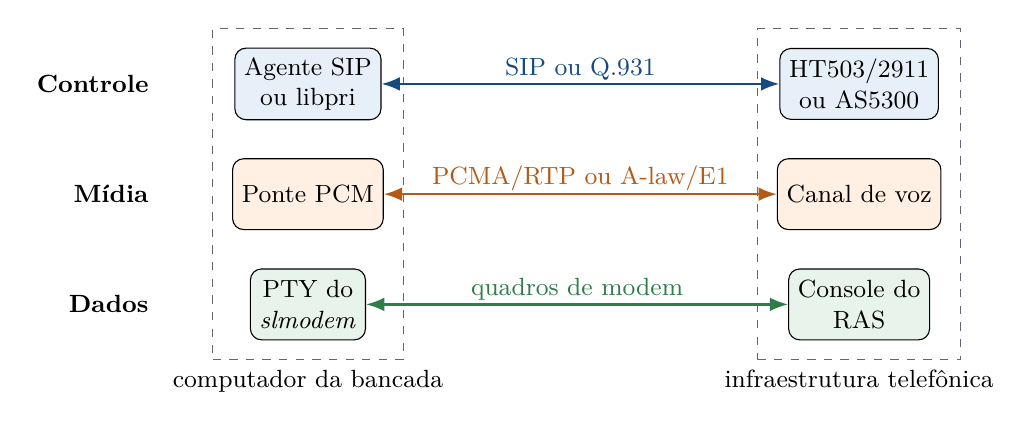
\begin{tikzpicture}[
  box/.style={draw,rounded corners,minimum height=0.9cm,align=center,font=\small},
  lab/.style={font=\small\bfseries,anchor=east},
  conn/.style={font=\small,fill=white,inner xsep=4pt,inner ysep=1pt},
  arr/.style={<->,>=Latex,thick}
]
  \node[lab] at (-0.4,2.2) {Controle};
  \node[box,fill=azulclaro] (sip1) at (1.5,2.2) {Agente SIP\\ou libpri};
  \node[box,fill=azulclaro] (sip2) at (8.5,2.2) {HT503/2911\\ou AS5300};
  \draw[arr,azul] (sip1) -- node[above,conn]{SIP ou Q.931} (sip2);

  \node[lab] at (-0.4,0.8) {Mídia};
  \node[box,fill=laranjaclaro] (pcm1) at (1.5,0.8) {Ponte PCM};
  \node[box,fill=laranjaclaro] (pcm2) at (8.5,0.8) {Canal de voz};
  \draw[arr,laranja] (pcm1) -- node[above,conn]{PCMA/RTP ou A-law/E1} (pcm2);

  \node[lab] at (-0.4,-0.6) {Dados};
  \node[box,fill=verdeclaro] (pty) at (1.5,-0.6) {PTY do\\\slmodem};
  \node[box,fill=verdeclaro] (ras) at (8.5,-0.6) {Console do\\RAS};
  \draw[arr,verde] (pty) -- node[above,conn]{quadros de modem} (ras);

  \begin{scope}[on background layer]
    \node[draw=cinza,dashed,fit=(sip1)(pcm1)(pty),inner sep=7pt,
          label=below:{\small computador da bancada}] {};
    \node[draw=cinza,dashed,fit=(sip2)(pcm2)(ras),inner sep=7pt,
          label=below:{\small infraestrutura telefônica}] {};
  \end{scope}
\end{tikzpicture}
\caption{Separação entre controle de chamada, transporte de mídia e validação de dados.}
\label{fig:planos}
\end{figure}

\section{Materiais e métodos}

\subsection{Equipamentos}

\begin{table}[htbp]
\centering
\caption{Equipamentos e funções na bancada.}
\label{tab:equipamentos}
\begin{tabularx}{\textwidth}{p{0.29\textwidth}p{0.27\textwidth}Y}
\toprule
\textbf{Equipamento} & \textbf{Função} & \textbf{Observação experimental} \\
\midrule
Cisco AS5300 & Servidor de acesso remoto & Modems digitais MICA e terminação E1; destino das chamadas de dados. \\
Cisco 2911 & Gateway de voz & PVDM3, VWIC3-1MFT-T1/E1 e VIC3-4FXS; interliga PRI, portas analógicas e SIP. \\
Conexant CX93010 USB & Modem cliente de referência & Valida o RAS e o caminho telefônico sem envolver o DSP do \slmodem. \\
Grandstream HT503 & Ponte SIP--analógico & Porta FXO ligada a uma FXS do 2911; mídia PCMA a \SI{8}{kHz}. \\
Sangoma A102 & Interface E1 do computador & Permite que DAHDI/libpri liguem o \slmodem{} diretamente ao AS5300. \\
Computador Linux & Execução e instrumentação & Hospeda pontes C, \slmodem, \arquivo{dialbench}, logs e capturas. \\
\bottomrule
\end{tabularx}
\end{table}

A montagem física final é apresentada na \cref{fig:rack-bancada}. A disposição no
rack manteve próximos o servidor de acesso, o gateway e o computador de controle,
reduzindo o percurso do cabeamento usado nas diferentes topologias.

\begin{figure}[htbp]
\centering
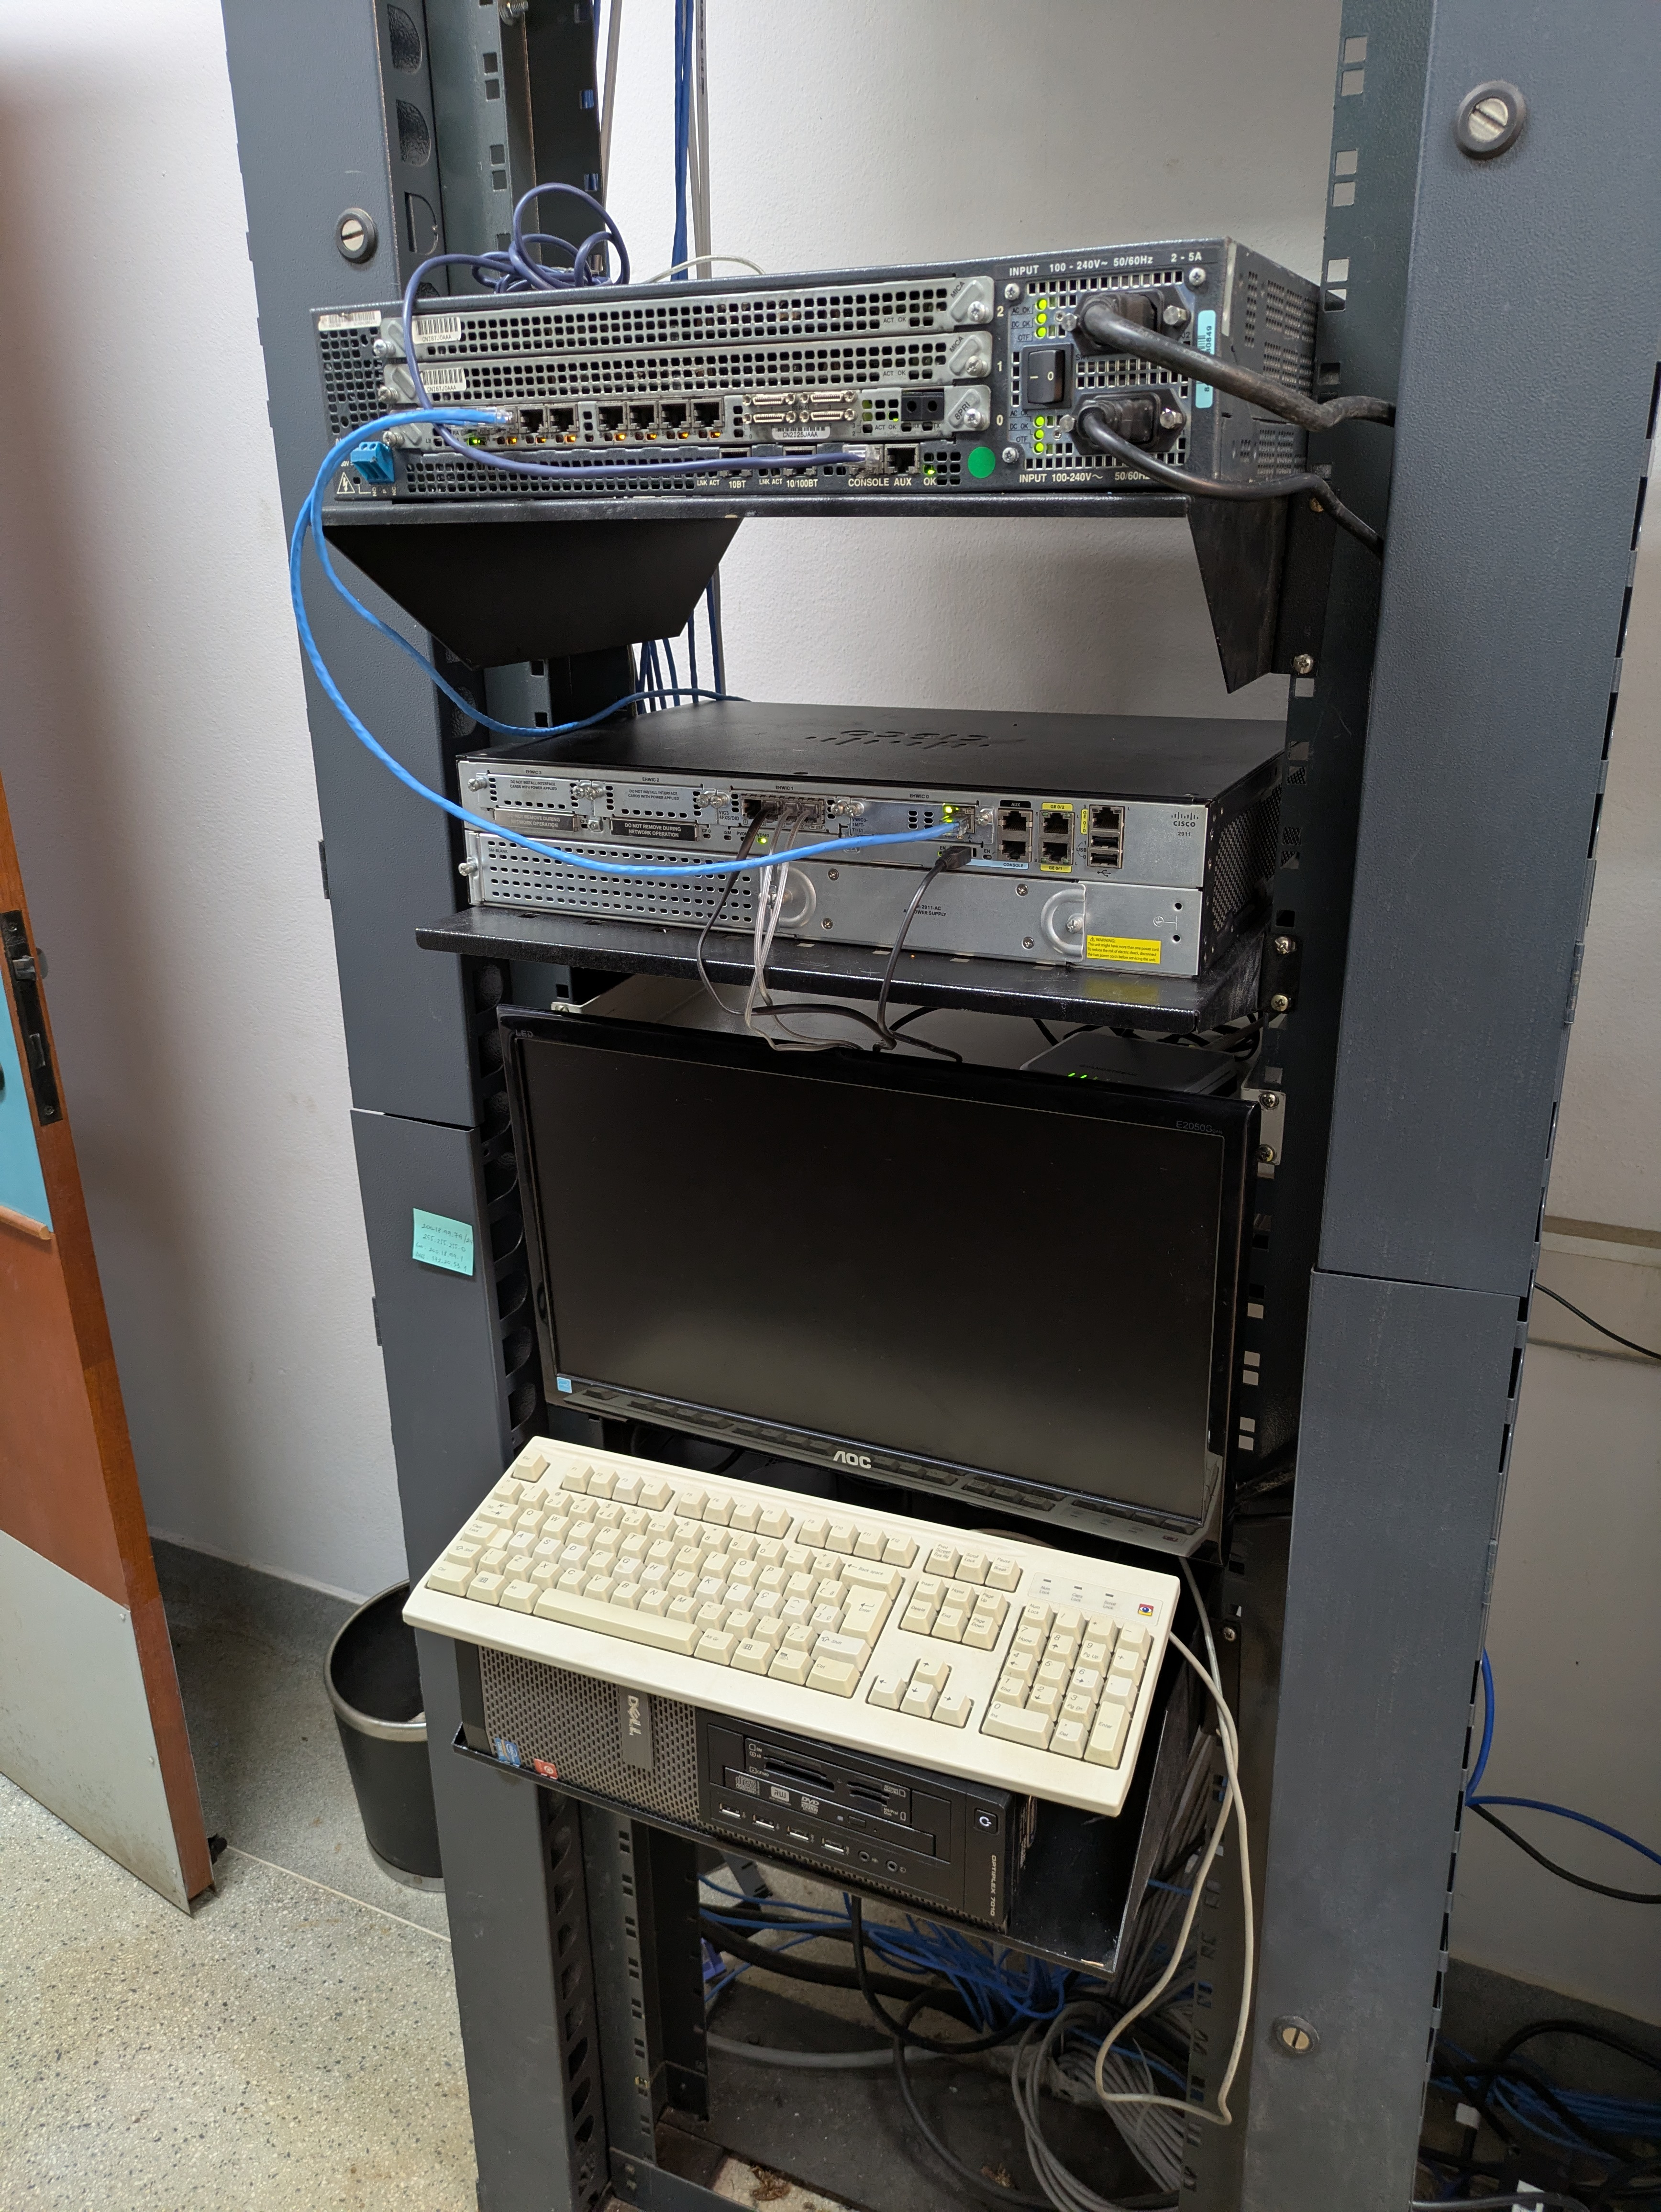
\includegraphics[height=0.57\textheight]{rack_bancada.jpg}
\caption[Montagem física da bancada no rack.]{Montagem física da bancada no
rack, com o servidor de acesso Cisco AS5300 na parte superior, o gateway Cisco
2911 ao centro e a estação de controle na parte inferior.}
\label{fig:rack-bancada}
\end{figure}
\FloatBarrier

\subsection{Topologias experimentais}

O plano aprovado continha três topologias incrementais. A quarta foi introduzida
durante a análise porque fornece o controle necessário para distinguir uma limitação
do transporte SIP de uma limitação da conversão analógica. A
\cref{fig:topologias} apresenta os quatro caminhos com a mesma convenção visual:
azul para transporte digital, laranja para conversão/linha analógica e verde para
os elementos terminais do teste.

\begin{figure}[p]
\centering
\begin{tikzpicture}[
  x=1cm,y=1cm,
  dev/.style={draw,rounded corners,thick,align=center,minimum height=0.95cm,
              text width=2cm,inner xsep=3pt,font=\footnotesize,fill=verdeclaro},
  net/.style={-{Latex[length=2.3mm]},thick,azul},
  ana/.style={-{Latex[length=2.3mm]},thick,laranja},
  rot/.style={font=\scriptsize,fill=white,inner xsep=2pt,inner ysep=0.5pt}
]
  \node[anchor=west,font=\bfseries\color{azul}] at (0,7.5) {Topologia 1 — validação com hardmodem};
  \node[dev] (pc1) at (1.1,6.4) {Computador};
  \node[dev] (hm1) at (5.35,6.4) {Conexant\\CX93010};
  \node[dev] (c1) at (9.6,6.4) {Cisco 2911\\FXS/PRI};
  \node[dev] (a1) at (13.85,6.4) {Cisco AS5300\\MICA};
  \draw[net] (pc1) -- node[rot]{USB} (hm1);
  \draw[ana] (hm1) -- node[rot]{linha} (c1);
  \draw[net] (c1) -- node[rot]{E1/PRI} (a1);

  \node[anchor=west,font=\bfseries\color{azul}] at (0,4.9) {Topologia 2 — \slmodem{} via HT503};
  \node[dev] (pc2) at (1.1,3.8) {\slmodem{} +\\ponte RTP};
  \node[dev,text width=2.2cm] (h2) at (5.35,3.8) {Grandstream\\HT503};
  \node[dev] (c2) at (9.6,3.8) {Cisco 2911\\FXS/PRI};
  \node[dev] (a2) at (13.85,3.8) {Cisco AS5300\\MICA};
  \draw[net] (pc2) -- node[rot]{SIP/RTP PCMA} (h2);
  \draw[ana] (h2) -- node[rot]{FXO--FXS} (c2);
  \draw[net] (c2) -- node[rot]{E1/PRI} (a2);

  \node[anchor=west,font=\bfseries\color{azul}] at (0,2.3) {Topologia 3 — E1 direto};
  \node[dev] (pc3) at (1.1,1.2) {\slmodem{} +\\\arquivo{pri_call}};
  \node[dev] (s3) at (7.475,1.2) {Sangoma A102\\DAHDI};
  \node[dev] (a3) at (13.85,1.2) {Cisco AS5300\\MICA};
  \draw[net] (pc3) -- node[rot]{PCM/A-law} (s3);
  \draw[net] (s3) -- node[rot]{E1/PRI} (a3);

  \node[anchor=west,font=\bfseries\color{azul}] at (0,-0.3) {Topologia 4 — controle SIP digital};
  \node[dev] (pc4) at (1.1,-1.4) {\slmodem{} +\\ponte RTP};
  \node[dev] (c4) at (7.475,-1.4) {Cisco 2911\\SIP/PRI};
  \node[dev] (a4) at (13.85,-1.4) {Cisco AS5300\\MICA};
  \draw[net] (pc4) -- node[rot]{SIP/RTP PCMA} (c4);
  \draw[net] (c4) -- node[rot]{E1/PRI} (a4);

  \begin{scope}[on background layer]
    \fill[laranjaclaro,rounded corners] ($(h2.south west)+(-0.2,-0.25)$)
      rectangle ($(c2.north east)+(0.2,0.25)$);
  \end{scope}
\end{tikzpicture}
\caption{Topologias avaliadas. A região laranja da topologia 2 é o trecho
analógico removido no controle da topologia 4.}
\label{fig:topologias}
\end{figure}

\paragraph{Topologia 1 — hardmodem.}
O computador controla o CX93010 por USB; a linha do modem chega a uma porta FXS
do 2911, e o gateway encaminha a chamada por PRI ao AS5300. O objetivo é estabelecer
uma referência independente do software cliente. Os ensaios foram conduzidos
manualmente pelo \texttt{picocom}: após o \texttt{CONNECT}, comandos eram enviados
ao RAS e suas respostas eram lidas pela própria conexão de dados.

\paragraph{Topologia 2 — SIP por meio do HT503.}
O \slmodem{} troca PCM com \arquivo{slmodem_bridge}; \arquivo{rtp_bridge} negocia
PCMA com o HT503. O número de destino aparece na URI SIP, e a porta FXO do ATA o
disca fisicamente na FXS do 2911. Esse caminho contém D/A, linha analógica e A/D.

\paragraph{Topologia 3 — E1 direto.}
O computador origina uma chamada EuroISDN por \arquivo{pri_call}. A Sangoma
recupera o relógio do AS5300, e as palavras A-law percorrem um domínio digital
síncrono. A topologia, originalmente opcional, tornou-se uma referência de alta
qualidade e de grande utilidade para V.90.

\paragraph{Topologia 4 — SIP digital.}
O Cisco 2911 recebe diretamente a chamada SIP, com PCMA, e encaminha a extensão 42
ao PRI. Mantêm-se \slmodem, SIP/RTP, PCMA, 2911, E1 e MICA, mas remove-se o HT503
e o trecho FXS/FXO. Assim, o contraste entre as topologias 2 e 4 isola o efeito
do caminho analógico, razão pela qual essa topologia adicional foi necessária.

\subsection{Arquitetura de software}

O software produzido reduz a adaptação do \slmodem{} a uma cadeia explícita de
processos. \arquivo{slmodem_bridge} liga o objeto de 32 bits, expõe uma PTY e
converte os quadros internos em PCM. \arquivo{rtp_bridge} estabelece SIP e
transporta PCMA; \arquivo{pri_call} estabelece Q.931 e transporta A-law por um
canal B DAHDI. O pacote Python \arquivo{dialbench} inicia os processos, conecta
seus fluxos, seleciona o protocolo e aplica o critério de aprovação. A arquitetura
é mostrada na \cref{fig:software}.

\begin{figure}[htbp]
\centering
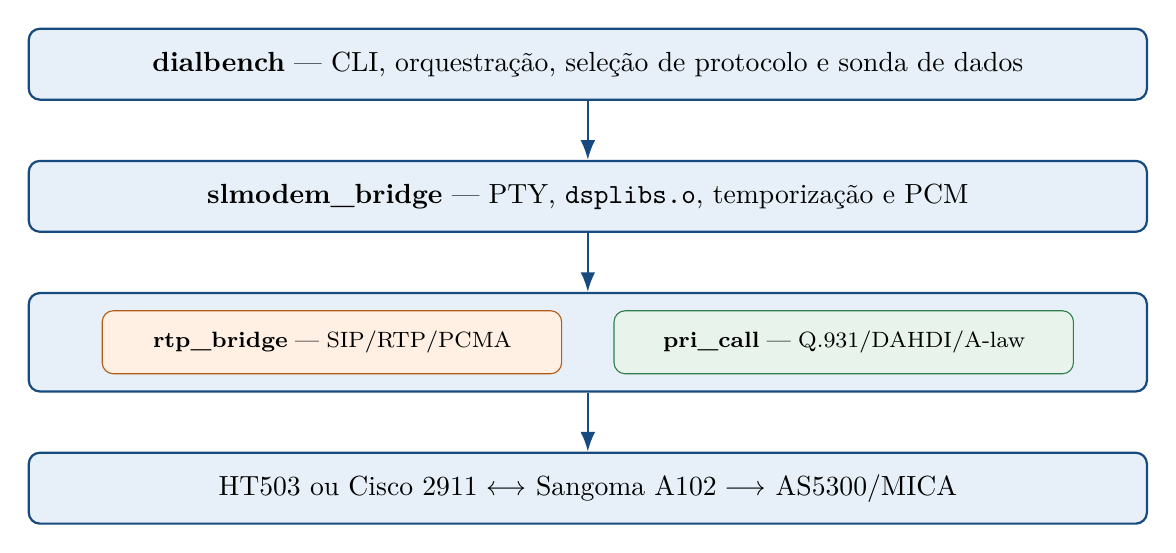
\begin{tikzpicture}[
  node distance=0.75cm,
  camada/.style={draw=azul,rounded corners,fill=azulclaro,thick,
                 minimum width=14.2cm,minimum height=0.9cm,align=center},
  transporte/.style={rounded corners,text width=5.6cm,minimum height=0.8cm,
                     align=center,font=\footnotesize},
  seta/.style={-{Latex[length=2.5mm]},thick,azul}
]
  \node[camada] (db) {\textbf{dialbench} — CLI, orquestração, seleção de protocolo e sonda de dados};
  \node[camada,below=of db] (slm) {\textbf{slmodem\_bridge} — PTY, \dsplibs, temporização e PCM};
  \node[camada,below=of slm,minimum height=1.25cm] (trans) {};
  \node[transporte,draw=laranja,fill=laranjaclaro]
        at ($(trans.center)+(-3.25,0)$) {\textbf{rtp\_bridge} — SIP/RTP/PCMA};
  \node[transporte,draw=verde,fill=verdeclaro]
        at ($(trans.center)+(3.25,0)$) {\textbf{pri\_call} — Q.931/DAHDI/A-law};
  \node[camada,below=of trans] (hw) {HT503 ou Cisco 2911 \hfill $\longleftrightarrow$ \hfill Sangoma A102 \hfill $\longrightarrow$ \hfill AS5300/MICA};
  \draw[seta] (db) -- (slm);
  \draw[seta] (slm) -- (trans);
  \draw[seta] (trans) -- (hw);
\end{tikzpicture}
\caption{Camadas do software desenvolvido para a bancada.}
\label{fig:software}
\end{figure}

Os \emph{data pumps} do binário trabalham em duas taxas. V.32/V.32bis possui
caminho nativo de \SI{8}{kHz}; os demais perfis usados na bancada operam a
\SI{9.6}{kHz}. Para estes, a conversão \SI{8}{kHz}$\leftrightarrow$\SI{9.6}{kHz}
usa o conversor \texttt{RcFixed}, reconstruído do objeto \texttt{dsplibs.o} original.
O valor \texttt{IODELAY} também faz parte do contrato: perfis
V.34/V.90 usam 240 amostras, enquanto V.32/V.32bis usa atraso zero.
Solicitações dinâmicas de ajuste de fila feitas pelo DSP são
honradas pelo wrapper.

\subsection{Critério de aprovação de uma chamada}

Uma indicação \texttt{CONNECT} prova apenas que uma fase local do modem reconheceu
portadora. Na topologia 1, a validação foi manual: o CX93010 foi operado pelo
\texttt{picocom} e, depois do estabelecimento da portadora, foram enviados comandos
ao AS5300 e lidas suas respostas. O V.90 também foi submetido a dois controles
adicionais: uma sessão permaneceu aberta por mais de \SI{24}{h}, e outra transportou
PPP entre o computador e o RAS, incluindo negociação IPCP e tráfego ICMP.

Nas topologias 2--4, o mesmo princípio foi automatizado. O \arquivo{dialbench}
espera a conexão, abre a PTY e envia \texttt{show clock} ao AS5300. A tentativa só
é aprovada quando recebe, na ordem, o eco do comando, uma linha com \texttt{UTC} e
o prompt \texttt{Router>}. Em regra foram exigidas três respostas completas;
algumas séries usaram 5, 12 ou 36 respostas para comprovar estabilidade em caminhos
que apresentaram problemas em algum estágio do desenvolvimento. O fluxo está na
\cref{fig:criterio}.

\begin{figure}[htbp]
\centering
\resizebox{\textwidth}{!}{%
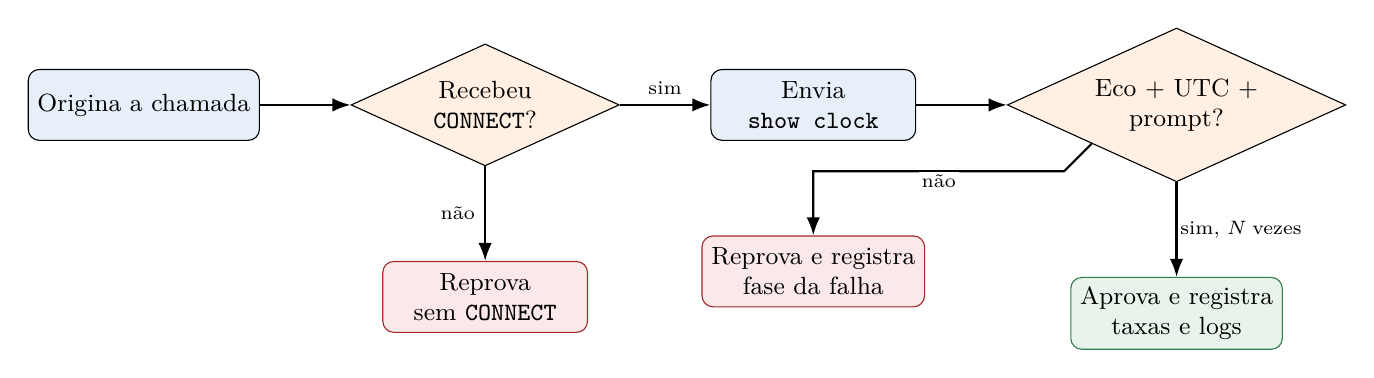
\begin{tikzpicture}[
  node distance=0.65cm and 1.15cm,
  proc/.style={draw,rounded corners,fill=azulclaro,minimum width=2.6cm,
               minimum height=0.9cm,align=center,font=\small},
  dec/.style={draw,diamond,aspect=2.2,fill=laranjaclaro,align=center,font=\small},
  arr/.style={-{Latex[length=2.3mm]},thick}
]
  \node[proc] (call) {Origina a chamada};
  \node[dec,right=of call] (conn) {Recebeu\\\texttt{CONNECT}?};
  \node[proc,right=of conn] (send) {Envia\\\texttt{show clock}};
  \node[dec,right=of send] (resp) {Eco + UTC +\\prompt?};
  \node[proc,below=1.2cm of resp,fill=verdeclaro,draw=verde] (pass) {Aprova e registra\\taxas e logs};
  \node[proc,below=1.2cm of conn,fill=vermelhoclaro,draw=vermelho] (fail1) {Reprova\\sem \texttt{CONNECT}};
  \node[proc,below=1.2cm of send,fill=vermelhoclaro,draw=vermelho] (fail2) {Reprova e registra\\fase da falha};
  \draw[arr] (call) -- (conn);
  \draw[arr] (conn) -- node[above,font=\scriptsize]{sim} (send);
  \draw[arr] (send) -- (resp);
  \draw[arr] (resp) -- node[right,font=\scriptsize,fill=white,inner sep=1pt]{sim, $N$ vezes} (pass);
  \draw[arr] (conn) -- node[left,font=\scriptsize]{não} (fail1);
  \draw[arr] (resp.south west) -- ++(-0.35,-0.35)
    -| node[pos=0.25,below,font=\scriptsize,fill=white,inner sep=1pt]{não} (fail2.north);
\end{tikzpicture}
}
\caption{Critério de validação de ponta a ponta utilizado nas topologias com \slmodem.}
\label{fig:criterio}
\end{figure}

\subsection{Ensaio de latência por eco}

Antes de integrar o modem, foi construído um ensaio simples para medir o custo do
caminho SIP/RTP e orientar a escolha da arquitetura. Primeiro, uma chamada com
\texttt{pjsua} reproduziu um arquivo de áudio pelo HT503 e comprovou o caminho
de sinalização e mídia. O ensaio foi então reformulado para medir o eco analógico
natural gerado na conversão de dois para quatro fios: a identidade da extremidade
distante não era importante, desde que o eco retornasse ao computador.

O estímulo final consiste em rajadas de seno a \SI{1}{kHz}, com \SI{100}{ms} de
duração e período de \SI{500}{ms}, amostradas a \SI{8}{kHz}. Um detector Goertzel
mede o início da rajada recebida; o intervalo é, portanto, um atraso de ida e volta
até o ponto de reflexão, e não uma latência unidirecional. O protótipo com baresip, PCMA e pacotes de
\SI{10}{ms} registrou 25 estimativas entre 89 e \SI{93}{ms}; depois da inclusão do
restante da cadeia, o valor observado ficou em torno de \SI{100}{ms}. Com buffers
de \emph{dejitter}, VAD e cancelamento de eco desativados, o pjsua ficou cerca de
\SI{20}{ms} acima desse valor. A ponte RTP própria, orientada a um único fluxo e
sem buffer de jitter, reduziu o atraso para aproximadamente \SI{70}{ms}.

Esses valores são registros de desenvolvimento, úteis para comparação arquitetural,
e não uma caracterização metrológica do atraso absoluto: o ponto de reflexão é um
eco do circuito analógico, e não foi preservada uma série bruta uniforme para as
três pilhas. Ainda assim, o resultado cumpriu sua finalidade de projeto: demonstrou
que a ponte enxuta tinha menor atraso e forneceu a base de código sobre a qual o
\slmodem{} foi integrado.

\begin{figure}[htbp]
\centering
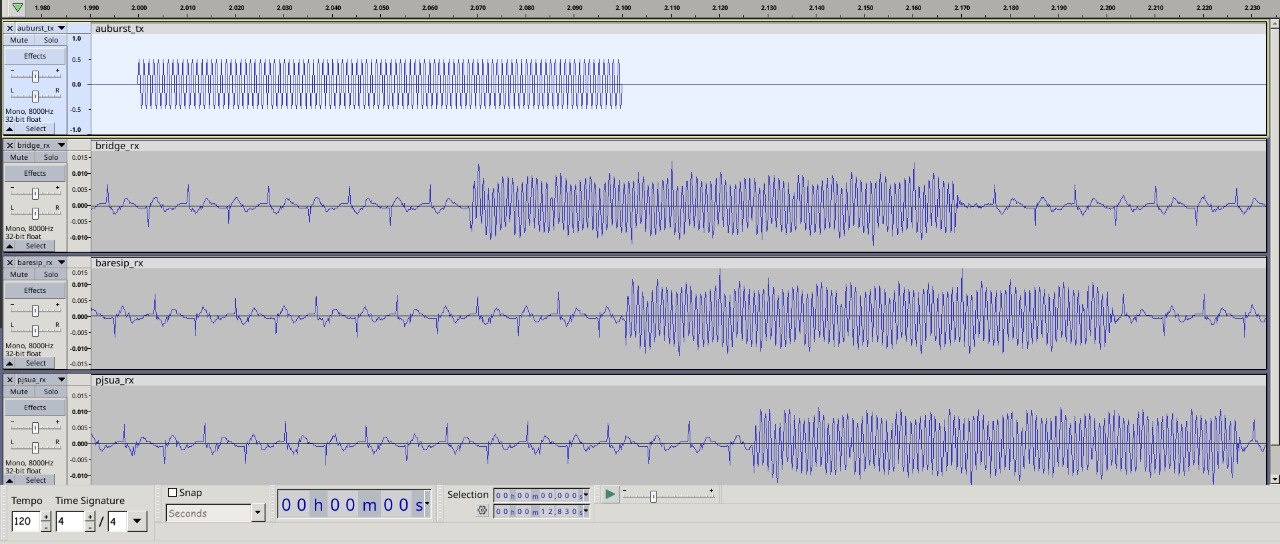
\includegraphics[width=0.90\textwidth]{latency_audacity.jpg}
\caption{Registro no Audacity com o estímulo e os retornos da ponte própria,
baresip e pjsua.}
\label{fig:latencia-registro}
\end{figure}

\begin{figure}[htbp]
\centering
  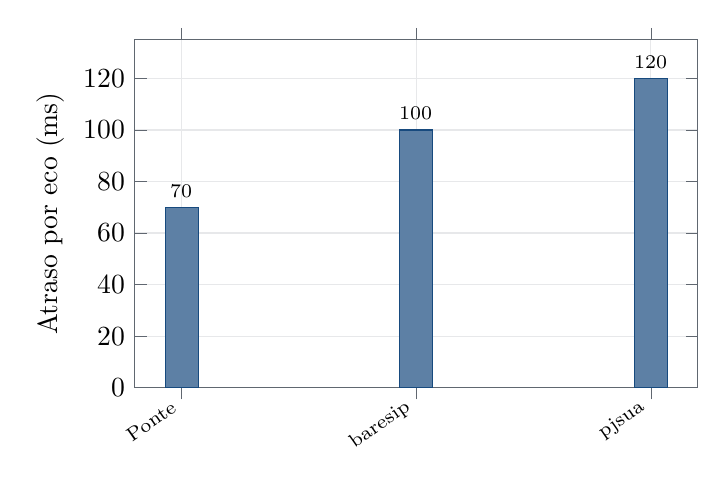
\begin{tikzpicture}
    \begin{axis}[
      ybar,bar width=12pt,
      width=0.72\textwidth,height=6.0cm,
      ymin=0,ymax=135,
      ylabel={Atraso por eco (ms)},
      symbolic x coords={Ponte,baresip,pjsua},
      xtick=data,
      x tick label style={rotate=35,anchor=east,font=\scriptsize},
      ytick distance=20,
      nodes near coords,
      nodes near coords style={font=\scriptsize},
      axis line style={cinza},
      tick style={cinza},
      grid=major,
      grid style={cinza!15}
    ]
      \addplot[fill=azul!70,draw=azul] coordinates {(Ponte,70) (baresip,100) (pjsua,120)};
    \end{axis}
  \end{tikzpicture}
\caption{Comparação aproximada do atraso por eco registrada durante a
prototipação, que orientou o desenvolvimento da ponte RTP dedicada.}
\label{fig:latencia-comparacao}
\end{figure}

\section{Desenvolvimento da bancada}

\subsection{Da chamada de áudio à integração do softmodem}

O desenvolvimento ocorreu por redução progressiva de incertezas. Primeiro foi
validada a sinalização SIP do HT503 e a reprodução de áudio com pjsua. Em seguida,
o ensaio de rajadas forneceu uma maneira objetiva de comparar o caminho crítico de
mídia. A observação de que um agente SIP genérico mantinha filas e serviços
desnecessários a uma única chamada motivou a criação de uma ponte dedicada. O SIP
permanece responsável pelo estabelecimento e encerramento, enquanto o fluxo RTP é
processado com o mínimo de cópias e sem buffer de \emph{dejitter} na LAN.

Com a ponte própria estabilizada em aproximadamente \SI{70}{ms}, o \slmodem{} foi
compilado em 32 bits e encapsulado. A primeira chamada funcional, em V.22 contra
um modem Conexant, confirmou a integração básica; os ensaios seguintes, com V.22bis
e V.32, revelaram erros HDLC. Esse comportamento levou à revisão da taxa de
amostragem, da conversão
\SI{8}{kHz}$\leftrightarrow$\SI{9.6}{kHz}, do empacotamento e dos pedidos de atraso
do DSP.

\subsection{Implementação do caminho E1}

A interface E1 direta, prevista como opcional, foi priorizada por eliminar a
conversão analógica e permitir uma referência síncrona. A primeira versão estabelecia
Q.931, mas falhava até em V.21. A comparação dos WAVs E1 e SIP mostrou que o
\slmodem{} produzia a mesma portadora correta; a divergência ocorria depois do ponto
de captura. O canal B estava aberto em modo não bloqueante e escritas que recebiam
\texttt{EAGAIN} eram descartadas. Além disso, a leitura em rajadas de até 1024
amostras fazia o modem produzir vários quadros de \SI{10}{ms} mais rapidamente que
a pequena fila DAHDI podia aceitá-los.

A correção acumulou exatamente 160 bytes PCM por quadro de 80 amostras A-law e
passou a respeitar o ritmo do canal. O controle V.21 permaneceu estável por
\SI{145.8}{s} e retornou dados do console. Nos protocolos mais rápidos, foram ainda
necessários: usar o conversor \texttt{RcFixed}; declarar corretamente o atraso
inicial; honrar \texttt{UPDATE\_DELAY}; e selecionar o perfil nativo de \SI{8}{kHz}
para V.32/V.32bis. Essas correções resultaram no conjunto de parâmetros indicado
na \cref{tab:perfis}.

\begin{table}[htbp]
\centering
\caption{Perfis finais de temporização do wrapper do \slmodem.}
\label{tab:perfis}
\begin{tabularx}{\textwidth}{p{0.36\textwidth}p{0.28\textwidth}Y}
\toprule
\textbf{Família} & \textbf{Taxa interna} & \textbf{Atraso inicial declarado} \\
\midrule
V.32 e V.32bis & \SI{8}{kHz} & \texttt{IODELAY=0} \\
V.21, V.22, V.22bis, V.23, V.34 e V.90 & \SI{9.6}{kHz}, com \texttt{RcFixed} & \texttt{IODELAY=240} \\
\bottomrule
\end{tabularx}
\end{table}

\subsection{Automação e reprodutibilidade}

O código inicialmente experimental foi organizado como o pacote
\arquivo{dialbench}. Cada transporte implementa uma interface de chamada; a CLI
seleciona modulação, taxa, atraso, portas SIP/RTP, canal B e quantidade de sondas.
Resultados consolidados foram gravados em \arquivo{tests/topologyN/results.csv}, e
as descrições de topologia registram os comandos, rotas, critérios e limitações.
Essa organização permite repetir um teste sem reconstruir manualmente a sequência
de processos ou interpretar \texttt{CONNECT} como sucesso suficiente. O código,
as instruções e as matrizes estão disponíveis em \repositorio.

Com os dois transportes estabilizados, a validação passou de chamadas isoladas para
uma matriz sistemática. O hardmodem confirmou o funcionamento do caminho telefônico
até V.90; o \slmodem{} passou por todos os protocolos no E1 direto e alcançou V.34
no caminho SIP por meio do HT503. Como apenas o V.90 falhava nesse último percurso,
o problema deixou de parecer uma deficiência geral de sinalização, mídia ou
integração e passou a exigir um experimento capaz de isolar o trecho analógico.

Essa necessidade levou à topologia 4. O novo controle preservou o \slmodem{},
SIP/RTP, PCMA, o Cisco 2911, E1/PRI e os modems MICA, retirando somente o HT503 e a
conversão FXS--FXO. O sucesso do V.90 nesse caminho mostrou que o transporte SIP
digital era adequado e direcionou a investigação para a resposta espectral, a
diferença entre relógios e a convergência do equalizador no trecho analógico. A
topologia adicional surgiu, portanto, como consequência lógica dos resultados da
matriz, e não como uma frente independente do desenvolvimento.

\section{Resultados}

\subsection{Matriz consolidada de protocolos}

A \cref{tab:matriz} reúne todos os protocolos registrados. TX e RX são dados da
perspectiva do cliente; em V.90, portanto, RX corresponde ao enlace descendente de
maior taxa. As topologias 2--4 só recebem aprovação quando completam a sonda
automatizada de dados. Na topologia 1, o critério equivalente foi aplicado
manualmente pelo \texttt{picocom}: além dos registros do hardmodem e do MICA,
houve envio de comandos ao RAS e leitura de suas respostas. Em V.90, a validação
incluiu ainda uma conexão PPP/IP e um ensaio prolongado de estabilidade.

\begin{landscape}
\begin{table}[p]
\centering
\caption{Matriz consolidada de conectividade e taxas negociadas.}
\label{tab:matriz}
\fontsize{10}{10.4}\selectfont
\renewcommand{\arraystretch}{0.95}
\begin{tabular}{C{1.1cm}lC{2.2cm}C{3.1cm}C{2.2cm}p{8.0cm}}
\toprule
\textbf{Top.} & \textbf{Protocolo} & \textbf{Resultado} & \textbf{TX/RX (bit/s)} & \textbf{Validação RAS} & \textbf{Observação} \\
\midrule
1 & V.21    & \ok & 300/300       & manual & Modem Conexant; comandos e respostas pelo \texttt{picocom}. \\
1 & V.22    & \ok & 1.200/1.200   & manual & LAPM/V.44; tráfego interativo. \\
1 & V.22bis & \ok & 2.400/2.400   & manual & LAPM/V.44; tráfego interativo. \\
1 & V.32bis & \ok & 14.400/14.400 & manual & Taxa integral; tráfego interativo. \\
1 & V.34    & \ok & 31.200/33.600 & manual & Assimetria negociada normal. \\
1 & V.90    & \ok & 31.200/46.667 & manual + PPP & IPCP e ICMP funcionais; sessão superior a \SI{24}{h}. \\
\midrule
2 & V.21    & \ok & 300/300       & 3/3  & \slmodem{} via HT503. \\
2 & V.22    & \ok & 1.200/1.200   & 3/3  & Tráfego bidirecional. \\
2 & V.22bis & \ok & 2.400/2.400   & 3/3  & Tráfego bidirecional. \\
2 & V.23    & \ok & 1.200/1.200   & 3/3  & Protocolo adicional ao plano. \\
2 & V.32bis & \ok & 14.400/14.400 & 36/36 & Doze chamadas; taxa integral. \\
2 & V.34    & \ok & 24.000/26.400 & 3/3  & Sem retransmissões observadas. \\
2 & V.90    & \falha & ---        & 0/3  & Falha de convergência na fase 4. \\
\midrule
3 & V.21    & \ok & 300/300       & 3/3  & E1 direto. \\
3 & V.22    & \ok & 1.200/1.200   & 3/3  & E1 direto. \\
3 & V.22bis & \ok & 2.400/2.400   & 3/3  & E1 direto. \\
3 & V.23    & \ok & 1.200/1.200   & 3/3  & E1 direto. \\
3 & V.32bis & \ok & 14.400/14.400 & 12/12 & Quatro chamadas. \\
3 & V.34    & \ok & 33.600/33.600 & 3/3  & Taxa máxima simétrica. \\
3 & V.90    & \ok & 31.200/56.000 & 5/5  & Taxa descendente máxima; dados reais. \\
\midrule
4 & V.21    & \ok & 300/300       & 3/3  & SIP/PCMA digital. \\
4 & V.22    & \ok & 1.200/1.200   & 3/3  & SIP/PCMA digital. \\
4 & V.22bis & \ok & 2.400/2.400   & 3/3  & SIP/PCMA digital. \\
4 & V.23    & \ok & 1.200/1.200   & 3/3  & Após estabilização de 10 s. \\
4 & V.32bis & \ok & 14.400/14.400 & 3/3  & Perfil nativo a \SI{8}{kHz}. \\
4 & V.34    & \ok & 31.200/33.600 & 3/3  & Portas SIP/RTP efêmeras. \\
4 & V.90    & \ok & \shortstack{26.400--28.800/\\54.667--56.000} & 3/3 por chamada & Quatro chamadas funcionais. \\
\bottomrule
\end{tabular}
\end{table}
\end{landscape}

O resultado central é que a bancada alcança todo o conjunto de protocolos até V.90
em três condições independentes: referência de hardware, E1 direto e SIP digital.
O único caso negativo é V.90 na topologia 2, enquanto todos os protocolos anteriores
passam no mesmo caminho. Isso afasta falhas gerais de roteamento, codec, chamada ou
integração do \slmodem{}.

\begin{figure}[htbp]
\centering
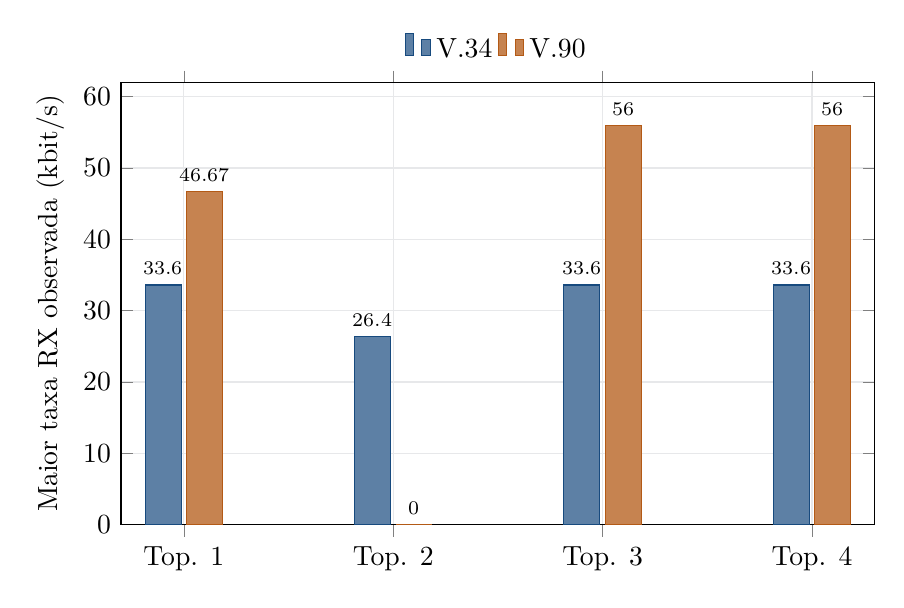
\begin{tikzpicture}
\begin{axis}[
  ybar,
  width=0.92\textwidth,height=7.2cm,
  ylabel={Maior taxa RX observada (kbit/s)},
  symbolic x coords={Top. 1,Top. 2,Top. 3,Top. 4},
  xtick=data,
  ymin=0,ymax=62,
  ytick distance=10,
  bar width=13pt,
  legend style={at={(0.5,1.02)},anchor=south,legend columns=2,draw=none},
  nodes near coords,
  nodes near coords style={font=\scriptsize},
  grid=major,grid style={cinza!15}
]
  \addplot[fill=azul!70,draw=azul] coordinates
    {(Top. 1,33.6) (Top. 2,26.4) (Top. 3,33.6) (Top. 4,33.6)};
  \addplot[fill=laranja!75,draw=laranja] coordinates
    {(Top. 1,46.667) (Top. 2,0) (Top. 3,56) (Top. 4,56)};
  \legend{V.34,V.90}
\end{axis}
\end{tikzpicture}
\caption{Taxas descendentes máximas observadas em V.34 e V.90. Zero indica
ausência de conexão V.90 funcional na topologia 2.}
\label{fig:taxas}
\end{figure}

\subsection{Topologia 1: referência com hardmodem}

O CX93010 conectou em todos os protocolos testados. Em V.90 negociou
\SI{31200}{bit/s} TX e \SI{46667}{bit/s} RX. A validação não se limitou à resposta
\texttt{CONNECT}: pelo \texttt{picocom}, foram enviados comandos ao RAS e recebidas
suas respostas. Uma das sessões V.90 permaneceu aberta por mais de \SI{24}{h}, sem
perda da portadora, demonstrando estabilidade prolongada do caminho de referência.

Também foi executado \texttt{pppd} sobre a porta serial do CX93010. LCP e IPCP
foram concluídos, atribuindo \texttt{192.168.7.100} ao cliente e
\texttt{192.168.7.25} ao RAS. Duas séries de dez mensagens ICMP não apresentaram
perdas; após ajustes nas configurações do Cisco 2911 e do RAS, o RTT médio caiu
de \SI{346.988}{ms} para \SI{124.562}{ms}, com redução simultânea da dispersão. A
\cref{tab:rtt-ppp} apresenta os valores registrados.

\begin{table}[htbp]
\centering
\caption{RTT ICMP sobre PPP na conexão V.90 da topologia 1.}
\label{tab:rtt-ppp}
\begin{tabular}{lS[table-format=3.3]S[table-format=3.3]S[table-format=3.3]S[table-format=2.3]c}
\toprule
\textbf{Condição} & {\textbf{Mín. (ms)}} & {\textbf{Média (ms)}} & {\textbf{Máx. (ms)}} & {\textbf{mdev (ms)}} & \textbf{Perda} \\
\midrule
Inicial     & 280.682 & 346.988 & 438.219 & 68.051 & 0/10 \\
Após ajuste & 110.996 & 124.562 & 159.320 & 12.528 & 0/10 \\
\bottomrule
\end{tabular}
\end{table}

Na visão do MICA, a mesma chamada aparecia como V.90 a
\SI{46666}{bit/s} TX e \SI{31200}{bit/s} RX, isto é, com os sentidos invertidos em
relação ao modem cliente, e relação sinal-ruído de \SI{39}{dB}. O equipamento
registrou ainda 41 pacotes PPP/SLIP transmitidos e 40 recebidos, nenhum pacote ruim
ou abortado e mais de dois mil caracteres em cada sentido. Seu indicador interno
\texttt{Round Trip Delay} marcou \SI{3}{ms}; ele caracteriza o enlace entre os
modems e não equivale ao RTT ICMP fim a fim da \cref{tab:rtt-ppp}, que inclui
serialização, filas e o processamento PPP nas duas extremidades.

Em conjunto, esses controles demonstram que os modems MICA, o AS5300, o PRI, o
2911 e a porta FXS sustentavam não apenas o treinamento V.90, mas uma sessão de
dados funcional e estável. Assim, falhas posteriores com o \slmodem{} não poderiam
ser atribuídas à configuração básica do RAS.

\subsection{Topologia 2: integração do HT503}

O objetivo de integrar o ATA foi alcançado: chamada, roteamento, áudio e dados
funcionaram de V.21 a V.34. V.32bis foi repetido em doze chamadas, totalizando 36
respostas válidas do RAS a \SI{14400}{bit/s} nos dois sentidos. V.34 negociou
\SI{24000}{bit/s} TX e \SI{26400}{bit/s} RX. V.90, contudo, não produziu
conexão de dados. A falha ocorre depois que o treinamento chega à fase 4, o que
motivou a investigação apresentada na \cref{sec:ht503}.

\subsection{Topologia 3: E1 direto}

Depois das correções de pacing e atraso, o E1 direto aprovou todos os protocolos.
Em V.90, a chamada de referência completou cinco de cinco sondas a
\SI{31200}{bit/s} TX e \SI{56000}{bit/s} RX, sem retransmissões. O
resultado cumpre a atividade opcional do projeto e fornece o caminho mais controlado
para futuros testes do \dsplibs: há quantização A-law na fronteira, porém não há
um segundo conversor analógico nem um relógio livre no percurso até o RAS.

É interessante introduzir esses elementos em ensaios futuros, pois seus efeitos
podem revelar defeitos que não aparecem no caminho digital controlado. Eles não
exigem, contudo, uma nova cadeia analógica física: conversão adicional, resposta em
frequência, ruído e diferença de relógio podem ser reproduzidos computacionalmente
por um simulador de linha. O desenvolvimento desse simulador foi considerado fora
do escopo da ICTSR, uma vez que o projeto submetido se comprometia apenas a avaliar
a viabilidade da conexão direta por E1. A topologia 3 estabelece, portanto, a base
experimental sobre a qual esse trabalho futuro poderá ser construído.

\subsection{Topologia 4: por que foi necessário um controle adicional}

A diferença entre topologias 2 e 3 removia simultaneamente HT503, SIP/RTP e Cisco
2911; por isso, não identificava qual elemento causava a falha. A topologia 4 foi
definida para manter SIP/RTP, PCMA e o gateway 2911, retirando somente a cadeia
FXS--FXO. O Cisco foi configurado para aceitar a extensão 42 por SIP e encaminhá-la
ao PRI com codec G.711 A-law e VAD desativado.

Quatro chamadas V.90 completaram as sondas; a última negociou
\SI{28800}{bit/s} TX e \SI{56000}{bit/s} RX após um retrain recuperável.
Foram recebidos 6092 pacotes RTP de 80 amostras, com timestamps contíguos. Portanto,
SIP, RTP, PCMA a \SI{8}{kHz} e o 2911 não são incompatíveis com V.90 quando carregam
diretamente a sequência PCM oriunda do E1. Esse controle é a ligação lógica entre a
matriz de conectividade e o diagnóstico do trecho analógico.

\section{Diagnóstico da limitação no caminho com HT503}
\label{sec:ht503}

\subsection{Estratégia de identificação}

Foram preservadas três capturas da sequência TRN1d: E1 direto, SIP digital e SIP
com a conversão analógica 2911--HT503. A análise reproduz exatamente o estimador de
espectro do receptor reconstruído, estima uma resposta FIR local do caminho adicional,
mede deriva temporal por correlação e aplica o mesmo núcleo de equalização a casos
fatoriais. O diagnóstico combina, portanto, quatro níveis de
evidência:

\begin{enumerate}
  \item chamadas de dados de ponta a ponta;
  \item capturas reais de áudio;
  \item reprodução dos critérios internos do binário;
  \item intervenção controlada que mascara apenas a primeira decisão de fallback.
\end{enumerate}

A captura E1 e a captura SIP digital contêm amostras TRN1d $\pm3904$ e apresentam
correlação normalizada 1,0 com 12000 símbolos reconstruídos. A
\cref{fig:trn1d} mostra a sequência, e a \cref{fig:rcfixed} apresenta a resposta
do conversor \texttt{RcFixed}.

\begin{figure}[htbp]
\centering
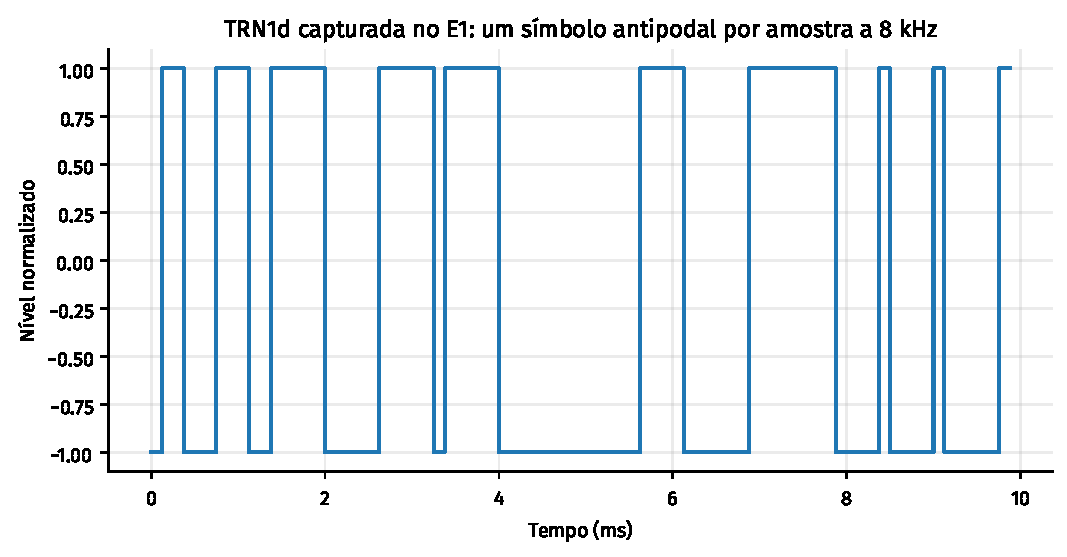
\includegraphics[width=0.88\textwidth]{trn1d_samples.pdf}
\caption{Amostras TRN1d capturadas no E1.}
\label{fig:trn1d}
\end{figure}

\begin{figure}[htbp]
\centering
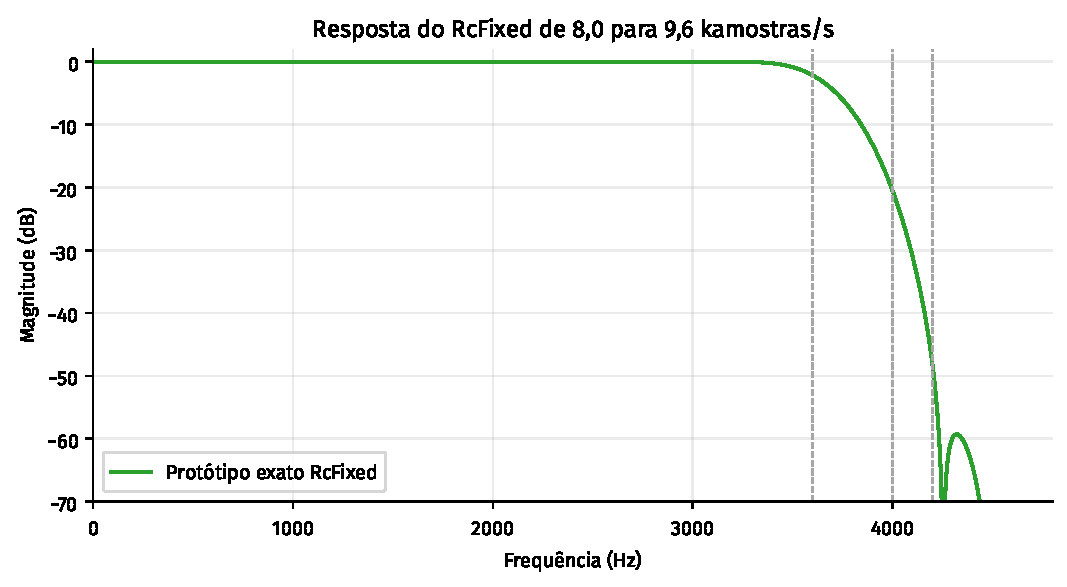
\includegraphics[width=0.88\textwidth]{rcfixed_response.pdf}
\caption{Resposta do conversor fixo de \SI{8}{kHz} para \SI{9.6}{kHz}.}
\label{fig:rcfixed}
\end{figure}

\FloatBarrier
\subsection{Resposta espectral medida}

O verificador de V.90 do \texttt{dsplibs.o} usa PSD de Welch a \SI{9.6}{kHz} e consulta
as regiões de \SI{3600}{Hz}, \SI{4000}{Hz} e \SI{4200}{Hz}. Ele classifica um codec como
severo somente quando as duas quedas em relação a \SI{3600}{Hz} excedem \SI{28}{dB}:

\begin{equation}
  \bigl[P(3600)-P(4000)>28\bigr]\ \land\
  \bigl[P(3600)-P(4200)>28\bigr].
  \label{eq:severo}
\end{equation}

Os valores medidos aparecem na \cref{tab:verificador}. E1 e SIP digital são quase
idênticos e não satisfazem a conjunção. O trecho analógico eleva ambas as quedas e
aciona o fallback.

\begin{table}[H]
\centering
\caption{Reprodução do verificador espectral com capturas da bancada.}
\label{tab:verificador}
\begin{tabular}{lrrrrl}
\toprule
\textbf{Caminho} & $P_{3600}$ & $P_{4000}$ & $P_{4200}$ & \multicolumn{1}{c}{$\Delta_{4000}/\Delta_{4200}$} & \textbf{Decisão} \\
 & \multicolumn{4}{c}{\si{dB}} & \\
\midrule
E1 digital & 96,220 & 76,185 & 47,501 & 20,036 / 48,719 & normal \\
SIP digital & 96,229 & 76,198 & 47,502 & 20,031 / 48,728 & normal \\
SIP D/A--A/D & 92,197 & 52,006 & 33,763 & 40,191 / 58,435 & severo \\
\bottomrule
\end{tabular}
\end{table}

Na escala do espectro completo, os dois caminhos digitais ficam sobrepostos na
\cref{fig:espectros}. As diferenças inferiores a \SI{0.01}{dB} na
\cref{tab:verificador} são compatíveis com pequenas variações de captura,
alinhamento e estimação entre ensaios independentes; sem uma série de repetições,
não lhes foi atribuído significado físico. A \cref{fig:verificador} mostra as
margens efetivamente relevantes para a decisão.

\begin{figure}[htbp]
\centering
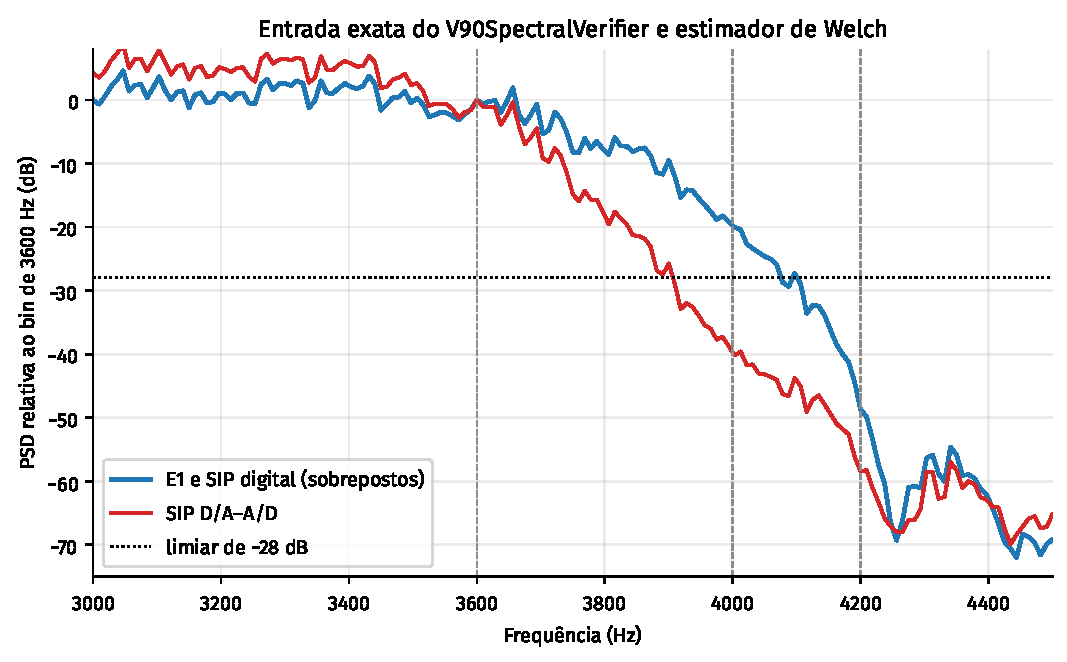
\includegraphics[width=0.92\textwidth]{measured_spectra.pdf}
\caption{Comparação espectral das rotas. E1 e SIP digital ficam sobrepostos na
escala relevante; a rota D/A--A/D apresenta a atenuação adicional.}
\label{fig:espectros}
\end{figure}

\begin{figure}[htbp]
\centering
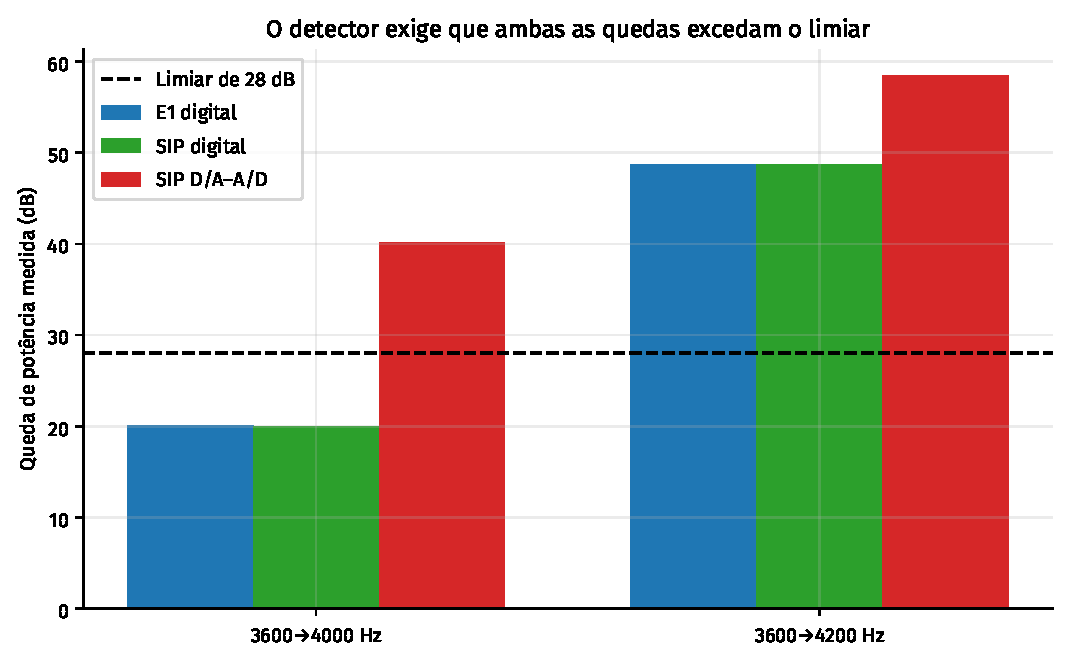
\includegraphics[width=0.84\textwidth]{verifier_budget.pdf}
\caption{Quedas medidas nas duas regiões de decisão. Somente a rota D/A--A/D
excede simultaneamente os dois limiares de \SI{28}{dB}.}
\label{fig:verificador}
\end{figure}

Modelos FIR de 80 coeficientes ajustados localmente ao trecho adicional atingiram
mediana $R^2=0{,}9811$ em dados reservados. A perda adicional, normalizada em
\SI{3600}{Hz}, foi \SI{10.065}{dB} em \SI{3800}{Hz} e \SI{21.025}{dB} em
\SI{3996}{Hz}. No controle SIP digital, as perdas correspondentes foram apenas
\SI{0.013}{dB} e \SI{0.032}{dB}. Isso fecha o orçamento espectral: a resposta medida
prediz, com erro inferior a \SI{1}{dB}, a mudança que faz o verificador classificar
o caminho como severo.

\FloatBarrier
\subsection{Relógios assíncronos e equalização}

A correlação em blocos encontrou deriva de $-0{,}913$ amostra por segundo no caminho
D/A--A/D, equivalente a \SI{-114.1}{ppm}; o SIP digital manteve offset constante e
deriva numericamente nula. A \cref{fig:resposta-canal} apresenta a resposta
adicional, e a \cref{fig:deriva-relogio}, o ajuste do relógio.

\begin{figure}[htbp]
\centering
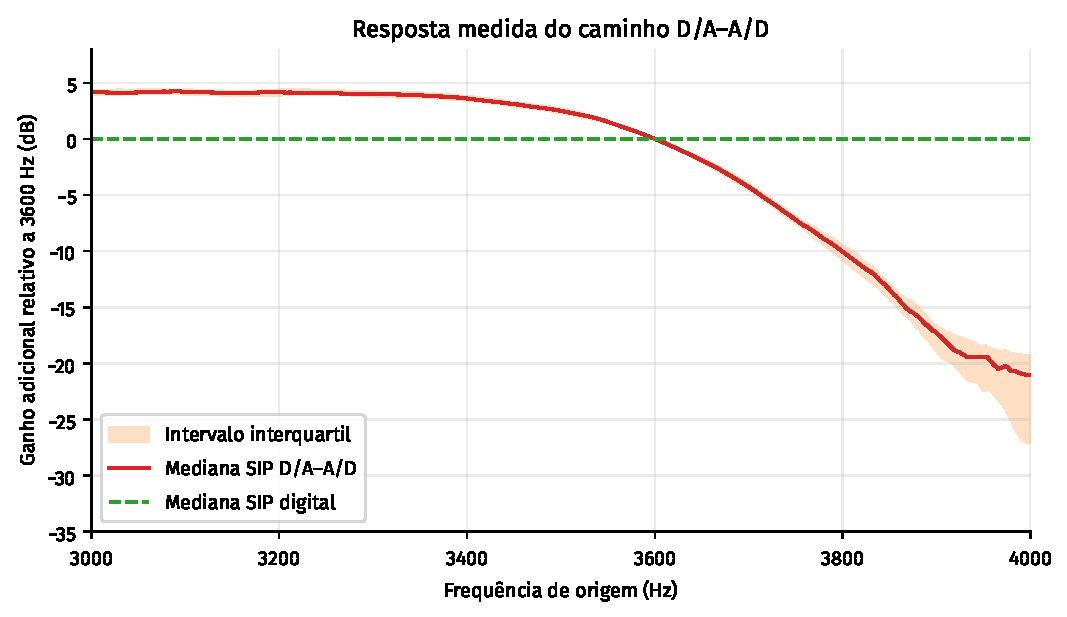
\includegraphics[width=0.88\textwidth]{channel_response.pdf}
\caption{Resposta do caminho adicional. A linha SIP digital funciona como
controle negativo para a perda em frequência.}
\label{fig:resposta-canal}
\end{figure}

\begin{figure}[htbp]
\centering
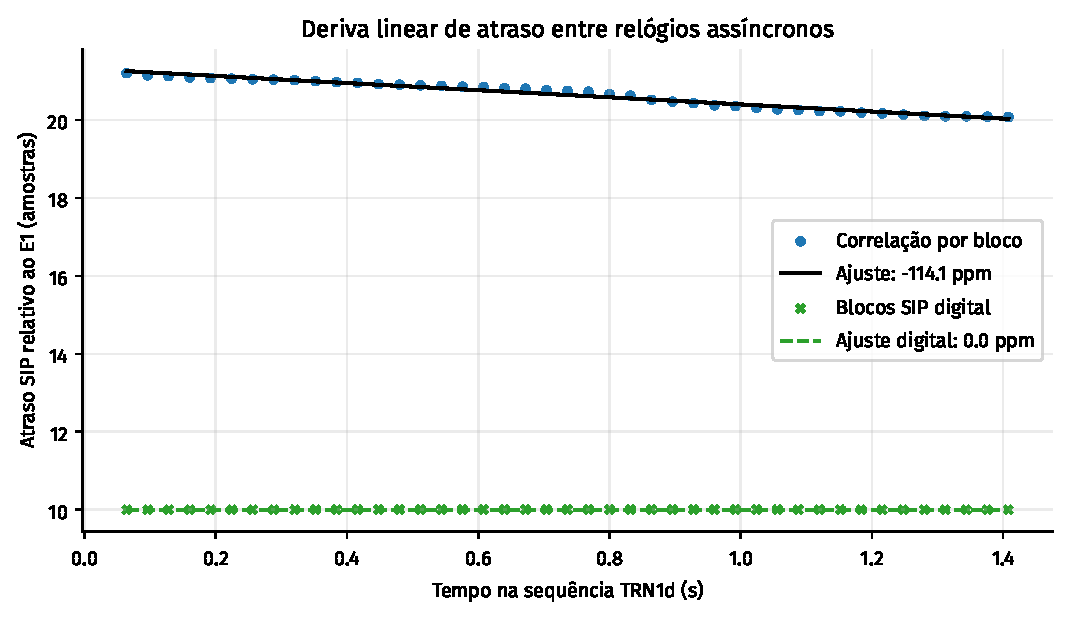
\includegraphics[width=0.88\textwidth]{clock_drift.pdf}
\caption{Deriva de amostragem medida. O SIP digital funciona como controle
negativo para a diferença entre relógios.}
\label{fig:deriva-relogio}
\end{figure}

O desvio de relógio não causa a decisão espectral, pois uma PSD é pouco sensível a
esse pequeno erro na janela usada. Simulações fatoriais confirmam que o filtro medido,
com ou sem desvio, cruza o limiar; o relógio isolado não. Nas etapas posteriores de
treinamento, entretanto, os efeitos interagem. A atenuação de borda reduz em cerca
de 127 vezes a componente de meia taxa usada pelo recuperador de temporização, que
deixa aproximadamente \SI{111.7}{ppm} sem compensação.

Ao final de TRN1d, o binário usa uma métrica média de erro, \texttt{avePdsnr}, com
limiar 180. O caso digital converge a 0 no modelo; o filtro medido com relógio
síncrono chega a 178,844, já marginal; filtro e relógio residual atingem 507,402.
A captura real resulta em 417,710, e mesmo após correção numérica completa do relógio
permanece em 397,319. A execução binária controlada mediu 359,076. Assim, o relógio
agrava a falha, mas sua correção isolada não recupera a informação espectral perdida.

\begin{figure}[htbp]
\centering
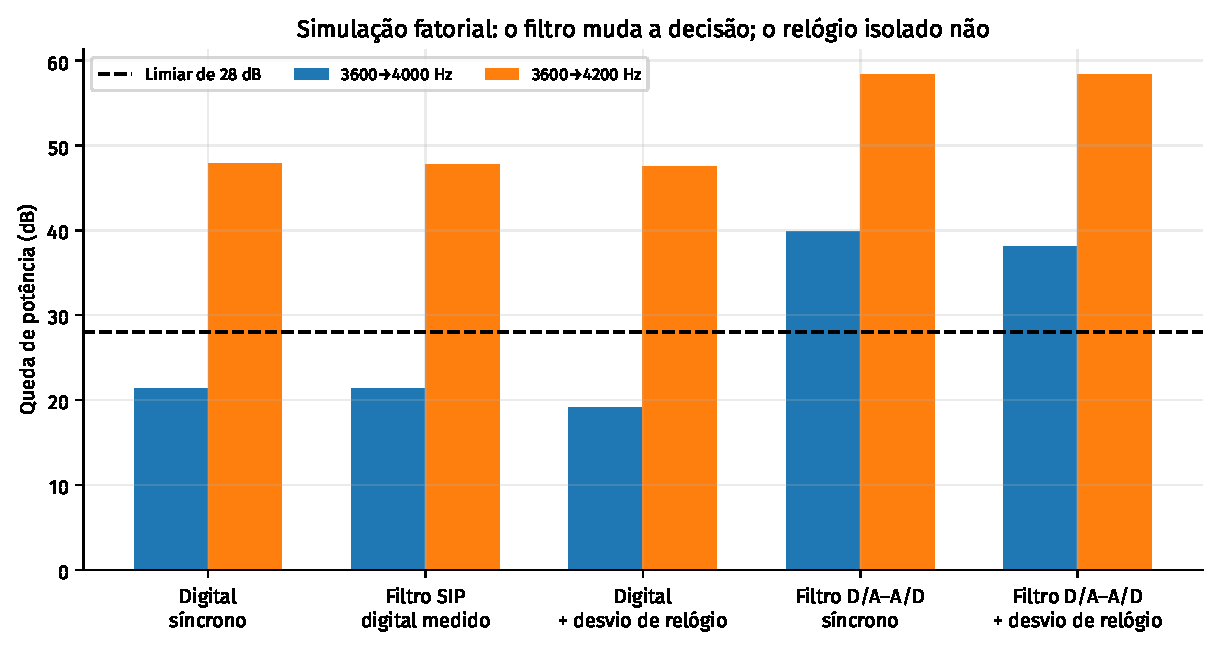
\includegraphics[width=0.92\textwidth]{filter_clock_factorial.pdf}
\caption{Decisão espectral sob fatores de filtro e relógio. O filtro explica a
decisão inicial, enquanto o desvio de relógio isolado não cruza o limiar.}
\label{fig:fatorial}
\end{figure}

\begin{figure}[htbp]
\centering
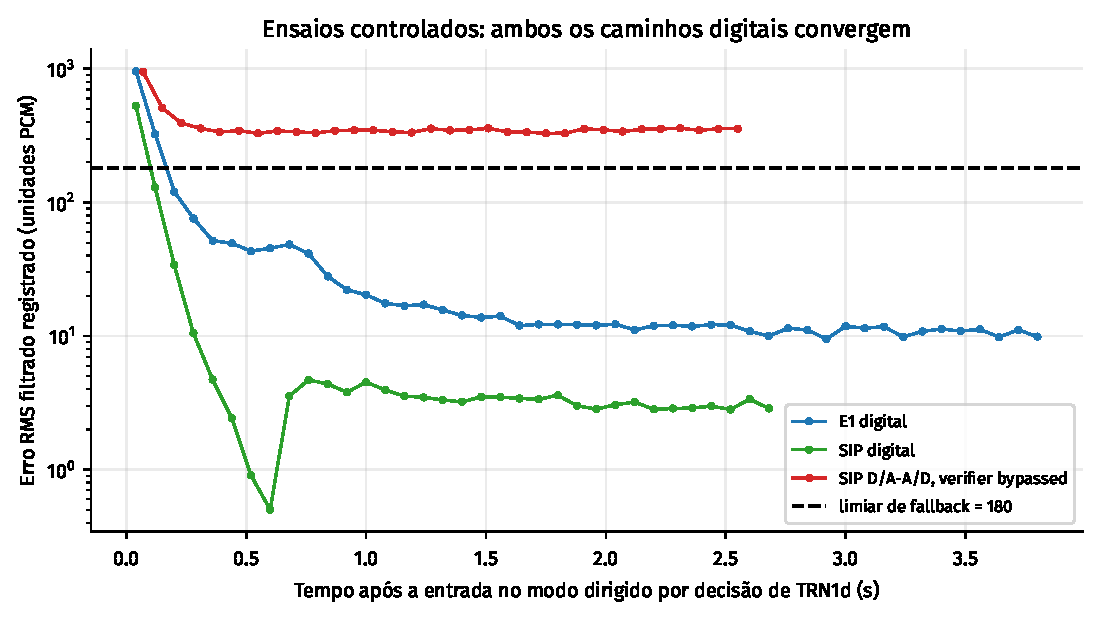
\includegraphics[width=0.88\textwidth]{bench_error_convergence.pdf}
\caption{Convergência da métrica registrada nos ensaios de bancada. Os dois
caminhos puramente digitais permanecem abaixo do limiar de fallback.}
\label{fig:convergencia-bancada}
\end{figure}

\begin{figure}[htbp]
\centering
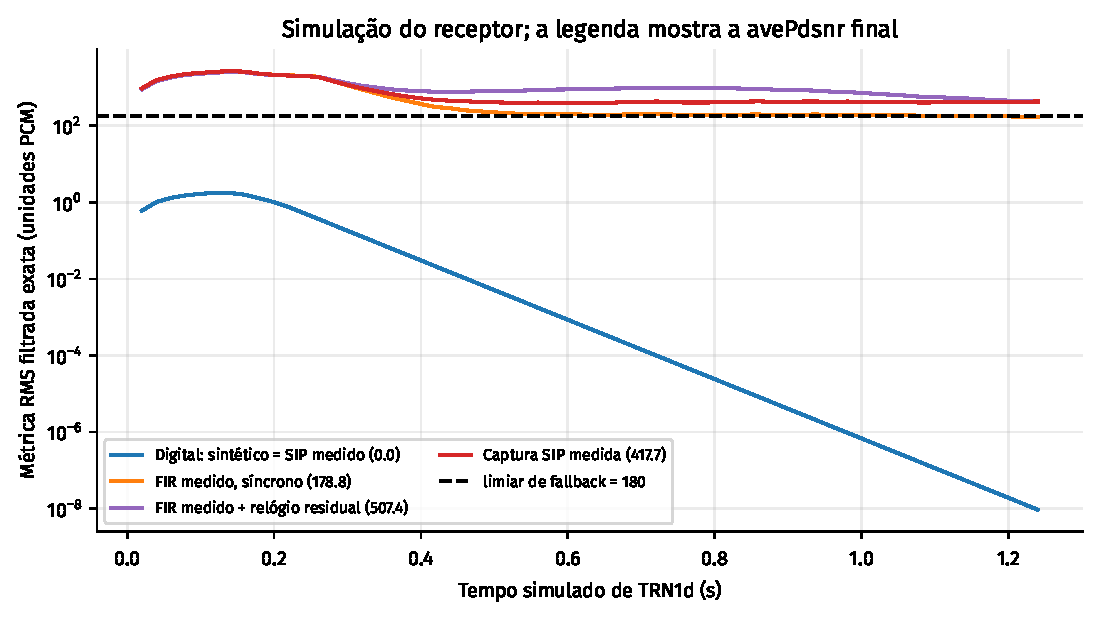
\includegraphics[width=0.88\textwidth]{ave_pdsnr_convergence.pdf}
\caption{Convergência no núcleo simulado. As trajetórias digital sintética e SIP
digital medida coincidem exatamente após o alinhamento; filtro e relógio residual
impedem a convergência posterior.}
\label{fig:convergencia}
\end{figure}

\FloatBarrier
\subsection{O que a documentação e a inspeção do HT503 acrescentam}

O HT503 contém um chipset VINETIC-2CPE/1CPE para o caminho analógico. A leitura da
documentação do fabricante e os ensaios exploratórios sustentam quatro conclusões,
ainda cautelosas quanto à implementação interna do componente:

\begin{itemize}
  \item \textbf{Separação funcional.} O processamento digital do módulo de linha
        analógica (ALM), denominado ACDSP nas interfaces de carregamento, é separado
        do EDSP, responsável por funções como codificação de voz e cancelamento de
        eco \cite{vinetic2006}.
  \item \textbf{Decimação.} No sentido linha--RTP, o manual situa o ADC sigma-delta
        de um bit, a redução da taxa de amostragem e os filtros programáveis antes da
        transferência ao EDSP. Ele não esclarece se o decimador é lógica dedicada ou
        parte do programa-base do ACDSP. Tampouco foi encontrada uma configuração
        funcional que alterasse a decimação do caminho FXO para operar acima de
        \SI{8}{kHz}.
  \item \textbf{Pré-filtro analógico.} Conversores sigma-delta empregam
        sobreamostragem seguida de filtragem digital e decimação, o que relaxa os
        requisitos do filtro anti-alias analógico \cite{pisani2023}. Assim, talvez
        o pré-filtro não seja o fator limitante.
  \item \textbf{Coeficientes BBD.} Os filtros do ACDSP recebem parâmetros de blocos
        BBD. Alterações preliminares elevaram a passagem em \SI{3.8}{kHz}, mas ainda
        não permitiram completar uma conexão V.90. A documentação pública não expõe
        a topologia matemática desses filtros nem o percurso exato do sinal entre
        seus estágios, portanto ainda não há base para propor um perfil definitivo.
\end{itemize}

A \cref{fig:vinetic-chain} resume apenas os blocos confirmados pela documentação.

\begin{figure}[htbp]
\centering
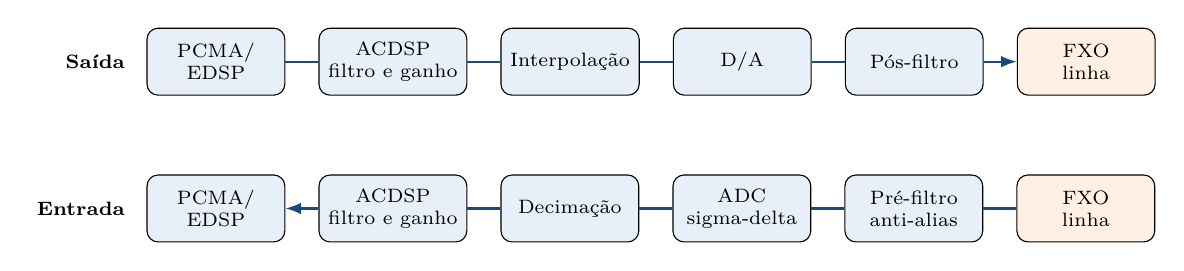
\begin{tikzpicture}[
  node distance=0.42cm,
  bloco/.style={draw,rounded corners,minimum width=1.75cm,minimum height=0.85cm,
                align=center,font=\scriptsize,fill=azulclaro},
  arr/.style={-{Latex[length=2mm]},thick,azul}
]
  \node[bloco] (pcm) {PCMA/\\EDSP};
  \node[bloco,right=of pcm] (lp) {ACDSP\\filtro e ganho};
  \node[bloco,right=of lp] (up) {Interpolação};
  \node[bloco,right=of up] (dac) {D/A};
  \node[bloco,right=of dac] (post) {Pós-filtro};
  \node[bloco,right=of post,fill=laranjaclaro] (line) {FXO\\linha};
  \draw[arr] (pcm)--(lp)--(up)--(dac)--(post)--(line);

  \node[bloco,below=1.0cm of pcm] (pcm2) {PCMA/\\EDSP};
  \node[bloco,right=of pcm2] (dig) {ACDSP\\filtro e ganho};
  \node[bloco,right=of dig] (down) {Decimação};
  \node[bloco,right=of down] (adc) {ADC\\sigma-delta};
  \node[bloco,right=of adc] (pre) {Pré-filtro\\anti-alias};
  \node[bloco,right=of pre,fill=laranjaclaro] (line2) {FXO\\linha};
  \draw[arr] (line2)--(pre)--(adc)--(down)--(dig)--(pcm2);
  \node[anchor=east,font=\scriptsize\bfseries] at ($(pcm.west)+(-0.15,0)$) {Saída};
  \node[anchor=east,font=\scriptsize\bfseries] at ($(pcm2.west)+(-0.15,0)$) {Entrada};
\end{tikzpicture}
\caption{Cadeias de sinal do módulo analógico VINETIC e separação funcional entre
ACDSP e EDSP, simplificadas a partir da documentação técnica.}
\label{fig:vinetic-chain}
\end{figure}

A própria especificação de resposta em frequência do VINETIC é esclarecedora. Entre
\SI{3}{kHz} e \SI{3.4}{kHz}, o fabricante limita a atenuação, relativa a
\SI{1}{kHz}, ao intervalo de \SI{-0.3}{dB} a \SI{1.7}{dB}. Entre
\SI{3.4}{kHz} e \SI{3.6}{kHz}, a máscara gráfica conserva apenas o limite inferior
de \SI{-0.3}{dB} de atenuação --- equivalente a limitar o ganho máximo a
\SI{0.3}{dB} --- e deixa de impor um limite superior para a atenuação. A tabela
correspondente tampouco especifica perda máxima acima de \SI{3.4}{kHz}, enquanto
\SI{3.8}{kHz} já está fora do domínio da figura. Portanto, o documento não garante
uma amplitude mínima na borda de banda de que o V.90 necessita. Isso não prova
sozinho a atenuação do aparelho; a prova quantitativa vem das capturas. A
especificação mostra, porém, que o resultado medido está fora da banda garantida,
não em contradição com ela.

\begin{figure}[htbp]
\centering
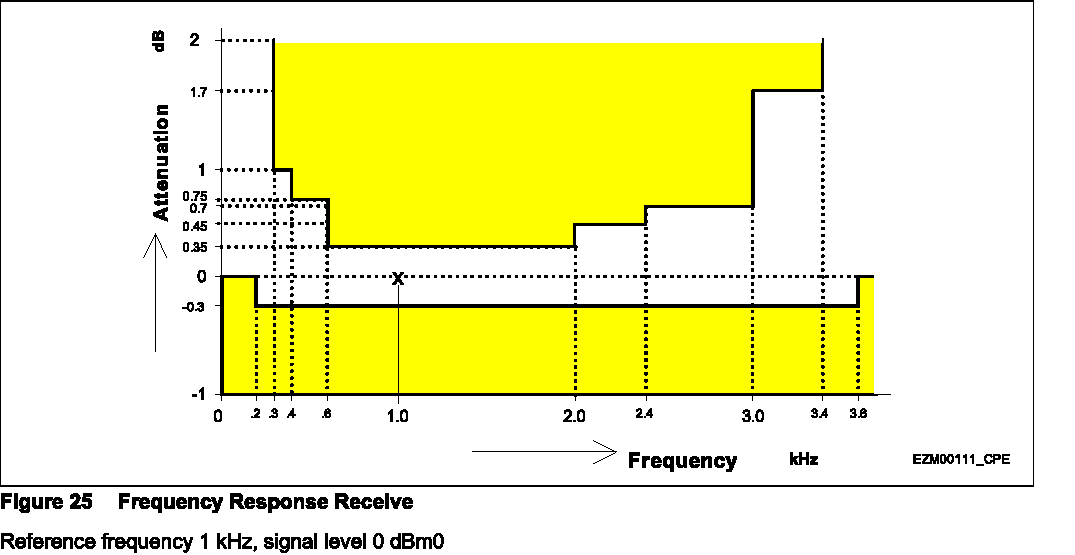
\includegraphics[width=0.92\textwidth]{vinetic_rx_freq_resp.pdf}
\caption[Limites documentados de resposta em frequência na recepção do VINETIC.]{Limites documentados de resposta em frequência na recepção do VINETIC.
De \SI{3}{kHz} a \SI{3.4}{kHz}, a máscara limita tanto o ganho quanto a atenuação;
entre \SI{3.4}{kHz} e \SI{3.6}{kHz}, permanece apenas o limite de ganho máximo,
sem limite de atenuação máxima. Em \SI{3.8}{kHz} não há especificação. Fonte: Infineon,
\emph{VINETIC CPE System Description}, rev. 1.1, figura 25, p. 65
\cite{vinetic2006}.}
\label{fig:vinetic-response}
\end{figure}

\FloatBarrier
\section{Discussão}

\subsection{Cumprimento do objetivo científico}

O objetivo não era obter sucesso incondicional em toda combinação imaginável de
equipamento, mas construir uma bancada que tornasse o comportamento do \slmodem{}
observável e verificável. Esse objetivo foi atingido em sentido mais forte que o
previsto: além de chamadas V.90 com hardmodem, o \slmodem{} alcançou
\SI{56000}{bit/s} em E1 direto e em SIP digital, com tráfego real. A topologia
opcional de E1 foi implementada; V.22bis e V.23 ampliaram a cobertura; e a falha do
HT503 foi transformada em resultado caracterizado por controles, espectro, relógio
e simulação.

A matriz de objetivos também evidencia competências típicas de iniciação científica
e tecnológica: leitura de documentação, montagem física, configuração de rede e
telefonia, programação de sistemas em C e Python, instrumentação, formulação de
hipóteses, comparação controlada, análise quantitativa e documentação reprodutível.
O trabalho não se resume a “fazer uma ligação”; ele estabelece uma metodologia para
detectar onde uma ligação falha e quais dados sustentam a conclusão.

\subsection{Interpretação correta da topologia 4}

A topologia 4 não constava do projeto porque sua necessidade só ficou visível depois
do resultado da topologia 2. Ela não representa mudança de tema. É um experimento
de controle: ao manter \slmodem, SIP/RTP, PCMA, Cisco 2911, PRI e AS5300, mas retirar
a conversão FXS/FXO, reduz o contraste a uma variável experimental relevante. Sem
ela, seria incorreto atribuir a falha ao ATA ou, no sentido oposto, ao transporte
SIP. Seu resultado positivo em V.90 é o principal suporte causal da discussão.

\subsection{Limitações}

O limite de atribuição deve ser explicitado. A captura não possui ponto de teste
calibrado entre a saída analógica do Cisco 2911 e a entrada do HT503. Portanto, a
resposta medida pertence ao trecho D/A--linha--A/D completo; não é possível dividir
com precisão os \SI{21}{dB} de perda entre os dois equipamentos. A documentação e
a inspeção do VINETIC explicam por que o HT503 não garante a banda requerida, mas
não tornam dispensável uma medição individual de cada conversor.

Os números de latência são comparações de prototipação. O método foi implementado e
o registro visual preservado, porém não há um conjunto homogêneo de WAVs e CSVs para
todas as três pilhas. Por isso, o relatório os apresenta como valores aproximados e
não calcula intervalos de confiança. Essa limitação não afeta a matriz de protocolos
nem a análise V.90, que possuem artefatos quantitativos próprios.

Por fim, ensaios preliminares com BBD mostraram que alterações de coeficientes afetam
a borda da banda, mas não identificaram as equações exatas nem produziram um perfil
estável para V.90. Essa limitação não impede que a bancada cumpra sua finalidade.

\section{Produtos e contribuições}

Os produtos diretamente utilizáveis após o encerramento do projeto são:

\begin{itemize}
  \item bancada física validada com RAS Cisco AS5300/MICA, gateway 2911, portas
        analógicas, SIP e E1 direto;
  \item \arquivo{tools/slmodem_bridge.c}, wrapper de 32 bits que expõe PTY e PCM;
  \item \arquivo{tools/rtp_bridge.c}, agente SIP e ponte RTP/PCMA de baixa latência;
  \item \arquivo{tools/pri_call.c}, originação Q.931 e transporte de canal B DAHDI;
  \item pacote \arquivo{dialbench}, com geração/análise de rajadas, callers, seleção
        de protocolo e sondas de dados;
  \item configurações e instruções para Cisco, DAHDI e Wanpipe;
  \item matrizes CSV e logs organizados por topologia;
  \item capturas WAV, scripts, tabelas e gráficos reprodutíveis do diagnóstico V.90;
  \item caracterização documentada da limitação do caminho analógico 2911--HT503;
  \item procedimento de controle SIP digital, que permite testar V.90 sem o ATA.
\end{itemize}

O repositório principal, disponível em \repositorio, conserva o histórico das decisões
de engenharia, o que permite que trabalhos posteriores repitam a bancada e avaliem
novas versões do \dsplibs{} reconstruído \cite{bancada}.

\section{Conclusões}

Foi construída uma bancada completa para testes de integração do \slmodem{} contra
um servidor de acesso real. O sistema combina controle de chamadas SIP e PRI,
transporte de áudio RTP/PCMA e E1/A-law, porta serial virtual, coleta de logs e uma
sonda que exige tráfego bidirecional antes de aprovar a conexão. O hardmodem de
referência validou o RAS até V.90. O \slmodem{} foi validado de V.21 a V.90 tanto no
E1 direto quanto no SIP digital, alcançando \SI{56000}{bit/s} no enlace
descendente.

O HT503 foi integrado com sucesso e suportou dados até V.34. Sua falha em V.90 não
invalidou a bancada; ao contrário, demonstrou a capacidade experimental criada.
A topologia 4 isolou o trecho analógico e provou que SIP/RTP/PCMA podem transportar
V.90 quando preservam a sequência PCM digital. As capturas quantificaram atenuação
adicional na borda da banda e um desvio de relógio de \SI{-114.1}{ppm}. A
documentação do VINETIC, que não limita a atenuação máxima acima de
\SI{3.4}{kHz}, e a ausência de um modo linear de banda larga habilitado no aparelho
são coerentes com o resultado.
Mascarar o primeiro fallback não recuperou a convergência, confirmando que a proteção
do modem detecta uma limitação real do canal.

As atividades previstas no projeto original foram executadas integralmente, inclusive
a etapa E1 inicialmente condicionada à disponibilidade de tempo e recursos. O
trabalho entregou infraestrutura, software, documentação, dados e um método objetivo
para validar as próximas funções reconstruídas do \dsplibs. O encerramento decorreu
da conclusão da graduação, e não de insuficiência técnica ou científica das
atividades.

\clearpage
\appendix

\section{Reprodução dos ensaios principais}

Os comandos abaixo registram a forma geral dos testes. Portas SIP/RTP podem ser
efêmeras; o canal B e o endereço do equipamento devem acompanhar a configuração
local.

\subsection{Construção das ferramentas}

\begin{lstlisting}[language=bash]
make -C tools
python3 -m dialbench --help
\end{lstlisting}

\subsection{Chamada pelo HT503}

\begin{lstlisting}[language=bash]
python3 -m dialbench modem slmodem_sip \
  --peer 'sip:42@10.42.0.102:5062;transport=udp' \
  -M 34 --probe-count 3
\end{lstlisting}

\subsection{Chamada por E1 direto}

\begin{lstlisting}[language=bash]
python3 -m dialbench modem slmodem_e1 \
  -M 90 --io-delay 240 --modem-rate 9600 \
  --probe-count 5
\end{lstlisting}

\subsection{Controle SIP digital}

\begin{lstlisting}[language=bash]
python3 -m dialbench modem slmodem_sip \
  --peer 'sip:42@10.42.0.22:5060;transport=udp' \
  --sip-port 0 --rtp-port 0 -M 90 \
  --io-delay 240 --modem-rate 9600 \
  --probe-count 3
\end{lstlisting}

\subsection{Análise do diagnóstico V.90}

\begin{lstlisting}[language=bash]
cd analysis/v90_sip
python3 -m venv .venv
.venv/bin/pip install -r requirements.txt
.venv/bin/python analyze.py
\end{lstlisting}

\section{Mapa dos artefatos}

Os caminhos da \cref{tab:artefatos} são relativos ao repositório público
\repositorio.

\begin{longtable}{p{0.38\textwidth}p{0.54\textwidth}}
\caption{Arquivos que sustentam os resultados do relatório.}
\label{tab:artefatos}\\
\toprule
\textbf{Caminho} & \textbf{Conteúdo} \\
\midrule
\endfirsthead
\toprule
\textbf{Caminho} & \textbf{Conteúdo} \\
\midrule
\endhead
\arquivo{tests/topology1/} & Procedimento, logs do hardmodem/AS5300 e matriz da topologia 1. \\
\arquivo{tests/topology2/} & Procedimento e matriz do \slmodem{} via HT503. \\
\arquivo{tests/topology3/} & Procedimento e matriz do E1 direto. \\
\arquivo{tests/topology4/} & Configuração, comandos e matriz do SIP digital. \\
\arquivo{docs/SLMODEM_NOTES.md} & Perfis de taxa, atraso, diagnósticos e regressões. \\
\arquivo{docs/dahdi.md} & Configuração da Sangoma, DAHDI e Wanpipe. \\
\arquivo{configs/} & Configurações sanitizadas e instruções de restauração da bancada. \\
\arquivo{dialbench/} & Orquestração, geração/análise de rajadas e sonda de dados. \\
\arquivo{tools/} & Pontes RTP, E1, baresip e \slmodem. \\
\arquivo{analysis/v90_sip/data/} & Três capturas TRN1d, chamada SIP digital completa, log e hashes. \\
\arquivo{analysis/v90_sip/results/} & CSVs e resumo numérico regenerados por \arquivo{analyze.py}. \\
\arquivo{analysis/v90_sip/analyze.py} & Análise reprodutível que também gera diretamente as figuras em \arquivo{docs/figures/}. \\
\bottomrule
\end{longtable}

\section{Protocolo, modulação e função no ensaio}

\begin{table}[H]
\centering
\caption{Protocolos empregados e progressão de complexidade.}
\begin{tabularx}{\textwidth}{lC{3cm}C{3.2cm}Y}
\toprule
\textbf{Protocolo} & \textbf{Taxa máxima} & \textbf{Modulação principal} & \textbf{Função no ensaio} \\
\midrule
V.21 & \SI{300}{bit/s} & FSK & Controle mínimo de sinalização e áudio bidirecional. \\
V.22 & \SI{1200}{bit/s} & PSK/DPSK & Introdução de portadora coerente e equalização. \\
V.22bis & \SI{2400}{bit/s} & QAM & Cobertura adicional e validação da progressão. \\
V.23 & \SI{1200}{bit/s} & FSK assimétrico & Cobertura adicional de data pump. \\
V.32bis & \SI{14400}{bit/s} & QAM + treliça & Cancelamento de eco e sensibilidade a atraso. \\
V.34 & \SI{33600}{bit/s} & QAM + treliça & Maior complexidade simétrica; limite funcional do HT503. \\
V.90 & 56/\SI{33.6}{kbit/s} & PCM desc./QAM asc. & Alvo principal; exige servidor com terminação digital. \\
\bottomrule
\end{tabularx}
\end{table}

\clearpage
\phantomsection
\addcontentsline{toc}{section}{Referências}
\bibliography{referencias}

\end{document}
